\documentclass{article}

% if you need to pass options to natbib, use, e.g.:
%     \PassOptionsToPackage{numbers, compress}{natbib}
% before loading neurips_data_2023

% ready for submission
% \usepackage{neurips_data_2023}

% to compile a preprint version, add the [preprint] option, e.g.:
%     \usepackage[preprint]{neurips_data_2023}
% This will indicate that the work is currently under review.

% to compile a camera-ready version, add the [final] option, e.g.:
\usepackage[final]{neurips_data_2023}

% to avoid loading the natbib package, add option nonatbib:
%    \usepackage[nonatbib]{neurips_data_2023}

% Submissions to the datasets and benchmarks are typically non anonymous,
% but anonymous submissions are allowed. If you feel that you must submit 
% anonymously, you can compile an anonymous version by adding the [anonymous] 
% option, e.g.:
%     \usepackage[anonymous]{neurips_data_2023}
% This will hide all author names.

\usepackage[utf8]{inputenc} % allow utf-8 input
\usepackage[T1]{fontenc}    % use 8-bit T1 fonts
\usepackage{hyperref}       % hyperlinks
\usepackage{url}            % simple URL typesetting
\usepackage{booktabs}       % professional-quality tables
\usepackage{amsfonts}       % blackboard math symbols
\usepackage{nicefrac}       % compact symbols for 1/2, etc.
\usepackage{microtype}      % microtypography
\usepackage{xcolor,colortbl}         % colors
\usepackage{adjustbox}
\usepackage{enumitem}
\usepackage{multicol}
\usepackage{multirow}
\usepackage{makecell}
\usepackage{soul}

\usepackage{amsmath}
\usepackage{amssymb}
\usepackage{mathtools}
\usepackage{amsthm}
\usepackage{bm}

\usepackage{siunitx} % symbols such as Angstrom notation
\DeclareSIUnit\angstrom{\text {Å}}  % enable latest support for Angstrom notation

%%%%% NEW MATH DEFINITIONS %%%%%

\usepackage{amsmath,amsfonts,bm}

% Mark sections of captions for referring to divisions of figures
\newcommand{\figleft}{{\em (Left)}}
\newcommand{\figcenter}{{\em (Center)}}
\newcommand{\figright}{{\em (Right)}}
\newcommand{\figtop}{{\em (Top)}}
\newcommand{\figbottom}{{\em (Bottom)}}
\newcommand{\captiona}{{\em (a)}}
\newcommand{\captionb}{{\em (b)}}
\newcommand{\captionc}{{\em (c)}}
\newcommand{\captiond}{{\em (d)}}

% Highlight a newly defined term
\newcommand{\newterm}[1]{{\bf #1}}


% Figure reference, lower-case.
\def\figref#1{figure~\ref{#1}}
% Figure reference, capital. For start of sentence
\def\Figref#1{Figure~\ref{#1}}
\def\twofigref#1#2{figures \ref{#1} and \ref{#2}}
\def\quadfigref#1#2#3#4{figures \ref{#1}, \ref{#2}, \ref{#3} and \ref{#4}}
% Section reference, lower-case.
\def\secref#1{section~\ref{#1}}
% Section reference, capital.
\def\Secref#1{Section~\ref{#1}}
% Reference to two sections.
\def\twosecrefs#1#2{sections \ref{#1} and \ref{#2}}
% Reference to three sections.
\def\secrefs#1#2#3{sections \ref{#1}, \ref{#2} and \ref{#3}}
% Reference to an equation, lower-case.
\def\eqref#1{equation~\ref{#1}}
% Reference to an equation, upper case
\def\Eqref#1{Equation~\ref{#1}}
% A raw reference to an equation---avoid using if possible
\def\plaineqref#1{\ref{#1}}
% Reference to a chapter, lower-case.
\def\chapref#1{chapter~\ref{#1}}
% Reference to an equation, upper case.
\def\Chapref#1{Chapter~\ref{#1}}
% Reference to a range of chapters
\def\rangechapref#1#2{chapters\ref{#1}--\ref{#2}}
% Reference to an algorithm, lower-case.
\def\algref#1{algorithm~\ref{#1}}
% Reference to an algorithm, upper case.
\def\Algref#1{Algorithm~\ref{#1}}
\def\twoalgref#1#2{algorithms \ref{#1} and \ref{#2}}
\def\Twoalgref#1#2{Algorithms \ref{#1} and \ref{#2}}
% Reference to a part, lower case
\def\partref#1{part~\ref{#1}}
% Reference to a part, upper case
\def\Partref#1{Part~\ref{#1}}
\def\twopartref#1#2{parts \ref{#1} and \ref{#2}}

\def\ceil#1{\lceil #1 \rceil}
\def\floor#1{\lfloor #1 \rfloor}
\def\1{\bm{1}}
\newcommand{\train}{\mathcal{D}}
\newcommand{\valid}{\mathcal{D_{\mathrm{valid}}}}
\newcommand{\test}{\mathcal{D_{\mathrm{test}}}}

\def\eps{{\epsilon}}


% Random variables
\def\reta{{\textnormal{$\eta$}}}
\def\ra{{\textnormal{a}}}
\def\rb{{\textnormal{b}}}
\def\rc{{\textnormal{c}}}
\def\rd{{\textnormal{d}}}
\def\re{{\textnormal{e}}}
\def\rf{{\textnormal{f}}}
\def\rg{{\textnormal{g}}}
\def\rh{{\textnormal{h}}}
\def\ri{{\textnormal{i}}}
\def\rj{{\textnormal{j}}}
\def\rk{{\textnormal{k}}}
\def\rl{{\textnormal{l}}}
% rm is already a command, just don't name any random variables m
\def\rn{{\textnormal{n}}}
\def\ro{{\textnormal{o}}}
\def\rp{{\textnormal{p}}}
\def\rq{{\textnormal{q}}}
\def\rr{{\textnormal{r}}}
\def\rs{{\textnormal{s}}}
\def\rt{{\textnormal{t}}}
\def\ru{{\textnormal{u}}}
\def\rv{{\textnormal{v}}}
\def\rw{{\textnormal{w}}}
\def\rx{{\textnormal{x}}}
\def\ry{{\textnormal{y}}}
\def\rz{{\textnormal{z}}}

% Random vectors
\def\rvepsilon{{\mathbf{\epsilon}}}
\def\rvtheta{{\mathbf{\theta}}}
\def\rva{{\mathbf{a}}}
\def\rvb{{\mathbf{b}}}
\def\rvc{{\mathbf{c}}}
\def\rvd{{\mathbf{d}}}
\def\rve{{\mathbf{e}}}
\def\rvf{{\mathbf{f}}}
\def\rvg{{\mathbf{g}}}
\def\rvh{{\mathbf{h}}}
\def\rvu{{\mathbf{i}}}
\def\rvj{{\mathbf{j}}}
\def\rvk{{\mathbf{k}}}
\def\rvl{{\mathbf{l}}}
\def\rvm{{\mathbf{m}}}
\def\rvn{{\mathbf{n}}}
\def\rvo{{\mathbf{o}}}
\def\rvp{{\mathbf{p}}}
\def\rvq{{\mathbf{q}}}
\def\rvr{{\mathbf{r}}}
\def\rvs{{\mathbf{s}}}
\def\rvt{{\mathbf{t}}}
\def\rvu{{\mathbf{u}}}
\def\rvv{{\mathbf{v}}}
\def\rvw{{\mathbf{w}}}
\def\rvx{{\mathbf{x}}}
\def\rvy{{\mathbf{y}}}
\def\rvz{{\mathbf{z}}}

% Elements of random vectors
\def\erva{{\textnormal{a}}}
\def\ervb{{\textnormal{b}}}
\def\ervc{{\textnormal{c}}}
\def\ervd{{\textnormal{d}}}
\def\erve{{\textnormal{e}}}
\def\ervf{{\textnormal{f}}}
\def\ervg{{\textnormal{g}}}
\def\ervh{{\textnormal{h}}}
\def\ervi{{\textnormal{i}}}
\def\ervj{{\textnormal{j}}}
\def\ervk{{\textnormal{k}}}
\def\ervl{{\textnormal{l}}}
\def\ervm{{\textnormal{m}}}
\def\ervn{{\textnormal{n}}}
\def\ervo{{\textnormal{o}}}
\def\ervp{{\textnormal{p}}}
\def\ervq{{\textnormal{q}}}
\def\ervr{{\textnormal{r}}}
\def\ervs{{\textnormal{s}}}
\def\ervt{{\textnormal{t}}}
\def\ervu{{\textnormal{u}}}
\def\ervv{{\textnormal{v}}}
\def\ervw{{\textnormal{w}}}
\def\ervx{{\textnormal{x}}}
\def\ervy{{\textnormal{y}}}
\def\ervz{{\textnormal{z}}}

% Random matrices
\def\rmA{{\mathbf{A}}}
\def\rmB{{\mathbf{B}}}
\def\rmC{{\mathbf{C}}}
\def\rmD{{\mathbf{D}}}
\def\rmE{{\mathbf{E}}}
\def\rmF{{\mathbf{F}}}
\def\rmG{{\mathbf{G}}}
\def\rmH{{\mathbf{H}}}
\def\rmI{{\mathbf{I}}}
\def\rmJ{{\mathbf{J}}}
\def\rmK{{\mathbf{K}}}
\def\rmL{{\mathbf{L}}}
\def\rmM{{\mathbf{M}}}
\def\rmN{{\mathbf{N}}}
\def\rmO{{\mathbf{O}}}
\def\rmP{{\mathbf{P}}}
\def\rmQ{{\mathbf{Q}}}
\def\rmR{{\mathbf{R}}}
\def\rmS{{\mathbf{S}}}
\def\rmT{{\mathbf{T}}}
\def\rmU{{\mathbf{U}}}
\def\rmV{{\mathbf{V}}}
\def\rmW{{\mathbf{W}}}
\def\rmX{{\mathbf{X}}}
\def\rmY{{\mathbf{Y}}}
\def\rmZ{{\mathbf{Z}}}

% Elements of random matrices
\def\ermA{{\textnormal{A}}}
\def\ermB{{\textnormal{B}}}
\def\ermC{{\textnormal{C}}}
\def\ermD{{\textnormal{D}}}
\def\ermE{{\textnormal{E}}}
\def\ermF{{\textnormal{F}}}
\def\ermG{{\textnormal{G}}}
\def\ermH{{\textnormal{H}}}
\def\ermI{{\textnormal{I}}}
\def\ermJ{{\textnormal{J}}}
\def\ermK{{\textnormal{K}}}
\def\ermL{{\textnormal{L}}}
\def\ermM{{\textnormal{M}}}
\def\ermN{{\textnormal{N}}}
\def\ermO{{\textnormal{O}}}
\def\ermP{{\textnormal{P}}}
\def\ermQ{{\textnormal{Q}}}
\def\ermR{{\textnormal{R}}}
\def\ermS{{\textnormal{S}}}
\def\ermT{{\textnormal{T}}}
\def\ermU{{\textnormal{U}}}
\def\ermV{{\textnormal{V}}}
\def\ermW{{\textnormal{W}}}
\def\ermX{{\textnormal{X}}}
\def\ermY{{\textnormal{Y}}}
\def\ermZ{{\textnormal{Z}}}

% Vectors
\def\vzero{{\bm{0}}}
\def\vone{{\bm{1}}}
\def\vmu{{\bm{\mu}}}
\def\vtheta{{\bm{\theta}}}
\def\va{{\bm{a}}}
\def\vb{{\bm{b}}}
\def\vc{{\bm{c}}}
\def\vd{{\bm{d}}}
\def\ve{{\bm{e}}}
\def\vf{{\bm{f}}}
\def\vg{{\bm{g}}}
\def\vh{{\bm{h}}}
\def\vi{{\bm{i}}}
\def\vj{{\bm{j}}}
\def\vk{{\bm{k}}}
\def\vl{{\bm{l}}}
\def\vm{{\bm{m}}}
\def\vn{{\bm{n}}}
\def\vo{{\bm{o}}}
\def\vp{{\bm{p}}}
\def\vq{{\bm{q}}}
\def\vr{{\bm{r}}}
\def\vs{{\bm{s}}}
\def\vt{{\bm{t}}}
\def\vu{{\bm{u}}}
\def\vv{{\bm{v}}}
\def\vw{{\bm{w}}}
\def\vx{{\bm{x}}}
\def\vy{{\bm{y}}}
\def\vz{{\bm{z}}}

% Elements of vectors
\def\evalpha{{\alpha}}
\def\evbeta{{\beta}}
\def\evepsilon{{\epsilon}}
\def\evlambda{{\lambda}}
\def\evomega{{\omega}}
\def\evmu{{\mu}}
\def\evpsi{{\psi}}
\def\evsigma{{\sigma}}
\def\evtheta{{\theta}}
\def\eva{{a}}
\def\evb{{b}}
\def\evc{{c}}
\def\evd{{d}}
\def\eve{{e}}
\def\evf{{f}}
\def\evg{{g}}
\def\evh{{h}}
\def\evi{{i}}
\def\evj{{j}}
\def\evk{{k}}
\def\evl{{l}}
\def\evm{{m}}
\def\evn{{n}}
\def\evo{{o}}
\def\evp{{p}}
\def\evq{{q}}
\def\evr{{r}}
\def\evs{{s}}
\def\evt{{t}}
\def\evu{{u}}
\def\evv{{v}}
\def\evw{{w}}
\def\evx{{x}}
\def\evy{{y}}
\def\evz{{z}}

% Matrix
\def\mA{{\bm{A}}}
\def\mB{{\bm{B}}}
\def\mC{{\bm{C}}}
\def\mD{{\bm{D}}}
\def\mE{{\bm{E}}}
\def\mF{{\bm{F}}}
\def\mG{{\bm{G}}}
\def\mH{{\bm{H}}}
\def\mI{{\bm{I}}}
\def\mJ{{\bm{J}}}
\def\mK{{\bm{K}}}
\def\mL{{\bm{L}}}
\def\mM{{\bm{M}}}
\def\mN{{\bm{N}}}
\def\mO{{\bm{O}}}
\def\mP{{\bm{P}}}
\def\mQ{{\bm{Q}}}
\def\mR{{\bm{R}}}
\def\mS{{\bm{S}}}
\def\mT{{\bm{T}}}
\def\mU{{\bm{U}}}
\def\mV{{\bm{V}}}
\def\mW{{\bm{W}}}
\def\mX{{\bm{X}}}
\def\mY{{\bm{Y}}}
\def\mZ{{\bm{Z}}}
\def\mBeta{{\bm{\beta}}}
\def\mPhi{{\bm{\Phi}}}
\def\mLambda{{\bm{\Lambda}}}
\def\mSigma{{\bm{\Sigma}}}

% Tensor
\DeclareMathAlphabet{\mathsfit}{\encodingdefault}{\sfdefault}{m}{sl}
\SetMathAlphabet{\mathsfit}{bold}{\encodingdefault}{\sfdefault}{bx}{n}
\newcommand{\tens}[1]{\bm{\mathsfit{#1}}}
\def\tA{{\tens{A}}}
\def\tB{{\tens{B}}}
\def\tC{{\tens{C}}}
\def\tD{{\tens{D}}}
\def\tE{{\tens{E}}}
\def\tF{{\tens{F}}}
\def\tG{{\tens{G}}}
\def\tH{{\tens{H}}}
\def\tI{{\tens{I}}}
\def\tJ{{\tens{J}}}
\def\tK{{\tens{K}}}
\def\tL{{\tens{L}}}
\def\tM{{\tens{M}}}
\def\tN{{\tens{N}}}
\def\tO{{\tens{O}}}
\def\tP{{\tens{P}}}
\def\tQ{{\tens{Q}}}
\def\tR{{\tens{R}}}
\def\tS{{\tens{S}}}
\def\tT{{\tens{T}}}
\def\tU{{\tens{U}}}
\def\tV{{\tens{V}}}
\def\tW{{\tens{W}}}
\def\tX{{\tens{X}}}
\def\tY{{\tens{Y}}}
\def\tZ{{\tens{Z}}}


% Graph
\def\gA{{\mathcal{A}}}
\def\gB{{\mathcal{B}}}
\def\gC{{\mathcal{C}}}
\def\gD{{\mathcal{D}}}
\def\gE{{\mathcal{E}}}
\def\gF{{\mathcal{F}}}
\def\gG{{\mathcal{G}}}
\def\gH{{\mathcal{H}}}
\def\gI{{\mathcal{I}}}
\def\gJ{{\mathcal{J}}}
\def\gK{{\mathcal{K}}}
\def\gL{{\mathcal{L}}}
\def\gM{{\mathcal{M}}}
\def\gN{{\mathcal{N}}}
\def\gO{{\mathcal{O}}}
\def\gP{{\mathcal{P}}}
\def\gQ{{\mathcal{Q}}}
\def\gR{{\mathcal{R}}}
\def\gS{{\mathcal{S}}}
\def\gT{{\mathcal{T}}}
\def\gU{{\mathcal{U}}}
\def\gV{{\mathcal{V}}}
\def\gW{{\mathcal{W}}}
\def\gX{{\mathcal{X}}}
\def\gY{{\mathcal{Y}}}
\def\gZ{{\mathcal{Z}}}

% Sets
\def\sA{{\mathbb{A}}}
\def\sB{{\mathbb{B}}}
\def\sC{{\mathbb{C}}}
\def\sD{{\mathbb{D}}}
% Don't use a set called E, because this would be the same as our symbol
% for expectation.
\def\sF{{\mathbb{F}}}
\def\sG{{\mathbb{G}}}
\def\sH{{\mathbb{H}}}
\def\sI{{\mathbb{I}}}
\def\sJ{{\mathbb{J}}}
\def\sK{{\mathbb{K}}}
\def\sL{{\mathbb{L}}}
\def\sM{{\mathbb{M}}}
\def\sN{{\mathbb{N}}}
\def\sO{{\mathbb{O}}}
\def\sP{{\mathbb{P}}}
\def\sQ{{\mathbb{Q}}}
\def\sR{{\mathbb{R}}}
\def\sS{{\mathbb{S}}}
\def\sT{{\mathbb{T}}}
\def\sU{{\mathbb{U}}}
\def\sV{{\mathbb{V}}}
\def\sW{{\mathbb{W}}}
\def\sX{{\mathbb{X}}}
\def\sY{{\mathbb{Y}}}
\def\sZ{{\mathbb{Z}}}

% Entries of a matrix
\def\emLambda{{\Lambda}}
\def\emA{{A}}
\def\emB{{B}}
\def\emC{{C}}
\def\emD{{D}}
\def\emE{{E}}
\def\emF{{F}}
\def\emG{{G}}
\def\emH{{H}}
\def\emI{{I}}
\def\emJ{{J}}
\def\emK{{K}}
\def\emL{{L}}
\def\emM{{M}}
\def\emN{{N}}
\def\emO{{O}}
\def\emP{{P}}
\def\emQ{{Q}}
\def\emR{{R}}
\def\emS{{S}}
\def\emT{{T}}
\def\emU{{U}}
\def\emV{{V}}
\def\emW{{W}}
\def\emX{{X}}
\def\emY{{Y}}
\def\emZ{{Z}}
\def\emSigma{{\Sigma}}

% entries of a tensor
% Same font as tensor, without \bm wrapper
\newcommand{\etens}[1]{\mathsfit{#1}}
\def\etLambda{{\etens{\Lambda}}}
\def\etA{{\etens{A}}}
\def\etB{{\etens{B}}}
\def\etC{{\etens{C}}}
\def\etD{{\etens{D}}}
\def\etE{{\etens{E}}}
\def\etF{{\etens{F}}}
\def\etG{{\etens{G}}}
\def\etH{{\etens{H}}}
\def\etI{{\etens{I}}}
\def\etJ{{\etens{J}}}
\def\etK{{\etens{K}}}
\def\etL{{\etens{L}}}
\def\etM{{\etens{M}}}
\def\etN{{\etens{N}}}
\def\etO{{\etens{O}}}
\def\etP{{\etens{P}}}
\def\etQ{{\etens{Q}}}
\def\etR{{\etens{R}}}
\def\etS{{\etens{S}}}
\def\etT{{\etens{T}}}
\def\etU{{\etens{U}}}
\def\etV{{\etens{V}}}
\def\etW{{\etens{W}}}
\def\etX{{\etens{X}}}
\def\etY{{\etens{Y}}}
\def\etZ{{\etens{Z}}}

% The true underlying data generating distribution
\newcommand{\pdata}{p_{\rm{data}}}
% The empirical distribution defined by the training set
\newcommand{\ptrain}{\hat{p}_{\rm{data}}}
\newcommand{\Ptrain}{\hat{P}_{\rm{data}}}
% The model distribution
\newcommand{\pmodel}{p_{\rm{model}}}
\newcommand{\Pmodel}{P_{\rm{model}}}
\newcommand{\ptildemodel}{\tilde{p}_{\rm{model}}}
% Stochastic autoencoder distributions
\newcommand{\pencode}{p_{\rm{encoder}}}
\newcommand{\pdecode}{p_{\rm{decoder}}}
\newcommand{\precons}{p_{\rm{reconstruct}}}

\newcommand{\laplace}{\mathrm{Laplace}} % Laplace distribution

\newcommand{\E}{\mathbb{E}}
\newcommand{\Ls}{\mathcal{L}}
\newcommand{\R}{\mathbb{R}}
\newcommand{\emp}{\tilde{p}}
\newcommand{\lr}{\alpha}
\newcommand{\reg}{\lambda}
\newcommand{\rect}{\mathrm{rectifier}}
\newcommand{\softmax}{\mathrm{softmax}}
\newcommand{\sigmoid}{\sigma}
\newcommand{\softplus}{\zeta}
\newcommand{\KL}{D_{\mathrm{KL}}}
\newcommand{\Var}{\mathrm{Var}}
\newcommand{\standarderror}{\mathrm{SE}}
\newcommand{\Cov}{\mathrm{Cov}}
% Wolfram Mathworld says $L^2$ is for function spaces and $\ell^2$ is for vectors
% But then they seem to use $L^2$ for vectors throughout the site, and so does
% wikipedia.
\newcommand{\normlzero}{L^0}
\newcommand{\normlone}{L^1}
\newcommand{\normltwo}{L^2}
\newcommand{\normlp}{L^p}
\newcommand{\normmax}{L^\infty}

\newcommand{\parents}{Pa} % See usage in notation.tex. Chosen to match Daphne's book.

\DeclareMathOperator*{\argmax}{arg\,max}
\DeclareMathOperator*{\argmin}{arg\,min}

\DeclareMathOperator{\sign}{sign}
\DeclareMathOperator{\Tr}{Tr}
\let\ab\allowbreak

\newcommand{\defeq}{\vcentcolon=}
\newcommand*{\ldblbrace}{\{\mskip-5mu\{}
\newcommand*{\rdblbrace}{\}\mskip-5mu\}}

\newcommand{\caa}{$C\alpha$ }
\newcommand{\virt}{$\kappa, \alpha$ }
\newcommand{\bb}{$\phi, \psi, \omega$ }
\newcommand{\schi}{$\chi_{1-4}$ }

\newcommand{\aj}[1]{\textcolor{red}{[\textbf{Arian}: #1]}}

\bibliographystyle{unsrtnat}
\setcitestyle{numbers,open={[},close={]},citesep={,}}

%\title{Evaluating Representation Learning on Protein Structures}
\title{Evaluating Representation Learning on \\ the Protein Structure Universe}

% The \author macro works with any number of authors. There are two commands
% used to separate the names and addresses of multiple authors: \And and \AND.
%
% Using \And between authors leaves it to LaTeX to determine where to break the
% lines. Using \AND forces a line break at that point. So, if LaTeX puts 3 of 4
% authors names on the first line, and the last on the second line, try using
% \AND instead of \And before the third author name.

% \author{%
%   Arian R. Jamasb$^*$ \\%\thanks{Use footnote for providing further information
%     %about author (webpage, alternative address)---\emph{not} for acknowledging
%     %funding agencies.} \\
%     %Department of Computer Science\\
%     University of Cambridge\\
%   \texttt{arj39@cam.ac.uk} \\
%   % examples of more authors
%   \And
%    Alex Morehead$^*$ \\
%    University of Missouri \\
%   % Address \\
%   \texttt{acmwhb@missouri.edu} \\
%     \AND
%     Zuobai Zhang$^*$ \\
%     Mila - Qu\'ebec AI Institute \\
%     \texttt{zuobai.zhang@mila.quebec} \\
%     \And
%     Chaitanya K. Joshi$^*$ \\
%     University of Cambridge \\
%     \texttt{ckj24@cam.ac.uk} \\
%     % Address \\
%     % \texttt{email} \\
%     \And
%     Kieran Didi \\
%     University of Cambridge \\
%     \texttt{ked48@cam.ac.uk} \\
%     \And
%     Simon Mathis \\
%     University of Cambridge \\
%     \texttt{svm34@cam.ac.uk} \\
%     \And
%     Charles Harris \\
%     University of Cambridge \\
%     \texttt{cch57@cam.ac.uk} \\
%     \And
%     Jian Tang \\
%     Mila - Qu\'ebec AI Institute \\
%     \texttt{jian.tang@hec.ca} \\
%     \And
%     Jianlin Cheng \\
%     University of Missouri \\
%     \texttt{chengji@missouri.edu} \\
%     \And
%     Pietro Lio \\
%     University of Cambridge \\
%     \texttt{pl219@cam.ac.uk}
%     \And
%     Tom L. Blundell \\
%     University of Cambridge \\
%    \texttt{tlb20@cam.ac.uk} \\
% }

\author{%
  Arian R. Jamasb$^{*,1}$, Alex Morehead$^{*,2}$, Zuobai Zhang$^{*,3}$, Chaitanya K. Joshi$^{*,1}$, \\ 
  \textbf{Kieran Didi$^{1}$, Simon Mathis$^{1}$, Charles Harris$^{1}$, Jian Tang$^{3}$, Jianlin Cheng$^{2}$,} \\ 
  \textbf{Pietro Liò$^{1}$, Tom L. Blundell$^{1}$} \\
  $^{1}$University of Cambridge \quad $^{2}$University of Missouri \quad $^{3}$Mila - Qu\'ebec AI Institute \\
  % \texttt{arj39@cam.ac.uk} % Emails can be added later!
}


\begin{document}

\maketitle

\begin{abstract}
% Protein structure representation learning is the foundation for promising applications in drug discovery, protein design, and function prediction.
% However, there remains a need for a robust, standardised benchmark to track the progress of new and established methods with greater granularity and relevance to downstream applications. 
We introduce \emph{ProteinWorkshop}, a comprehensive benchmark suite for Geometric Graph Neural Networks and protein structure representation learning.
% We provide large-scale pre-training and downstream tasks comprised of both experimental and predicted structures, offering a balanced challenge to representation learning algorithms. 
% These tasks enable the systematic evaluation of the quality of the learned embeddings, the structural and functional relationships captured, and their usefulness in downstream tasks. 
We consider large-scale pre-training and downstream tasks on both experimental and predicted structures to enable the systematic evaluation of the quality of the learned structural representation, the functional relationships captured, and their usefulness in downstream tasks. 
% We benchmark state-of-the-art protein-specific and generic geometric Graph Neural Networks and the extent to which they benefit from different types of pre-training. 
% We find that pre-training consistently improves the performance of both rotation-invariant and equivariant geometric models, and that equivariant models seem to benefit even more from pre-training compared to invariant models.
We find that: (1) large-scale pretraining on AlphaFold-predicted structures and auxiliary tasks consistently improve the performance of both rotation-invariant and equivariant Geometric GNNs, and (2) more expressive equivariant GNNs benefit from pretraining to a greater extent compared to invariant models.

We aim to establish a common ground for the machine learning and computational biology communities to rigorously compare and advance protein structure representation learning. 
% By providing a standardised and rigorous evaluation platform, we expect to accelerate the development of novel methodologies and improve our understanding of protein structures and their functions. 
Our open-source codebase reduces the barrier to entry for working with large protein structure datasets by providing: (1) storage-efficient dataloaders from large-scale predicted structures including AlphaFoldDB and ESM Atlas, as well as (2) utilities for constructing new tasks from the entire PDB.
\emph{ProteinWorkshop} is available at: \href{https://github.com/a-r-j/ProteinWorkshop}{\texttt{github.com/a-r-j/ProteinWorkshop}}.

% The codebase incorporates several engineering contributions which considerably reduces the barrier to entry for pre-training and working with large structure-based datasets. Our benchmark is available at: \url{https://anonymous.4open.science/r/ProteinWorkshop-B8F5}. 
%at \href{https://www.github.com/a-r-j/ProteinWorkshop}{\texttt{https://www.github.com/a-r-j/ProteinWorkshop}}.

\end{abstract}

\section{Introduction}

Modern protein structure prediction methods have led to an explosion in the availability of structural data \citep{jumper2021highly, baek2021accurate}. While many sequence-based functional annotations can be directly mapped to structures, this has resulted in a significantly-increasing gap between structures and meaningful \emph{structural} annotations \citep{Varadi2021}. Recent work has focused on developing methods to draw biological insights from large volumes of structural data by either determining representative structures that can be used to provide such annotations \citep{holm2022dali} or representing structures in a simplified and compact manner such as sequence alphabets \citep{vanKempen2023} or graph embeddings \citep{greener2022fast}. These works have significantly reduced the computational resources required to process and analyse such structural representatives at scale. Nonetheless, it remains to be shown how such results can help us better understand the relationship between protein sequence, structure, and function through the use of deep learning algorithms.

Several deep learning methods have been developed for protein structures. In particular, Geometric Graph Neural Networks (GNNs) \citep{duval2023hitchhiker} have emerged as the architecture of choice for learning structural representations of biomolecules \citep{schutt2018schnet, Gasteiger2020directional, jing2020learning, schutt2021equivariantmp, morehead2022geometric, zhang2023protein}.
Methods can be categorised according to (1) the featurisation schemes and level of granularity of input structures (C$\alpha$, backbones, all-atom); as well as (2) the enforcement of physical symmetries and inductive biases (invariant or equivariant representations) \citep{joshi2023expressive}.
However, there remains a need for a robust, standardised benchmark to track the progress of new and established methods with greater granularity and relevance to downstream applications. 

In this work, we develop a unified and rigorous framework for evaluating protein structural encoders, providing pretraining corpora that span known foldspace and tasks that assess the ability of models to learn informative representations at different levels of structural granularity. Previous works in protein structure representation learning have focused on learning effective \emph{global} (i.e. graph-level) representations of protein structure, typically evaluating the methods on function or fold classification tasks \citep{Gligorijevi2021, zhang2023protein}. However, there has been comparatively little investigation into the ability of different methods to learn informative local (\emph{node-level}) representations. Good node-level representations are important for a variety of annotation tasks, such as binding or interaction site prediction \citep{gainza2020deciphering}, as well as providing conditioning signals in structure-conditioned molecule design methods \citep{schneuing2022structure, corso2023diffdock}. Understanding the structure-function relationship at this granular level can drive progress in protein design by revealing structural motifs that underlie desirable properties, enabling them to be incorporated into designs.

%%%
\begin{figure}[t!]
    \centering
% 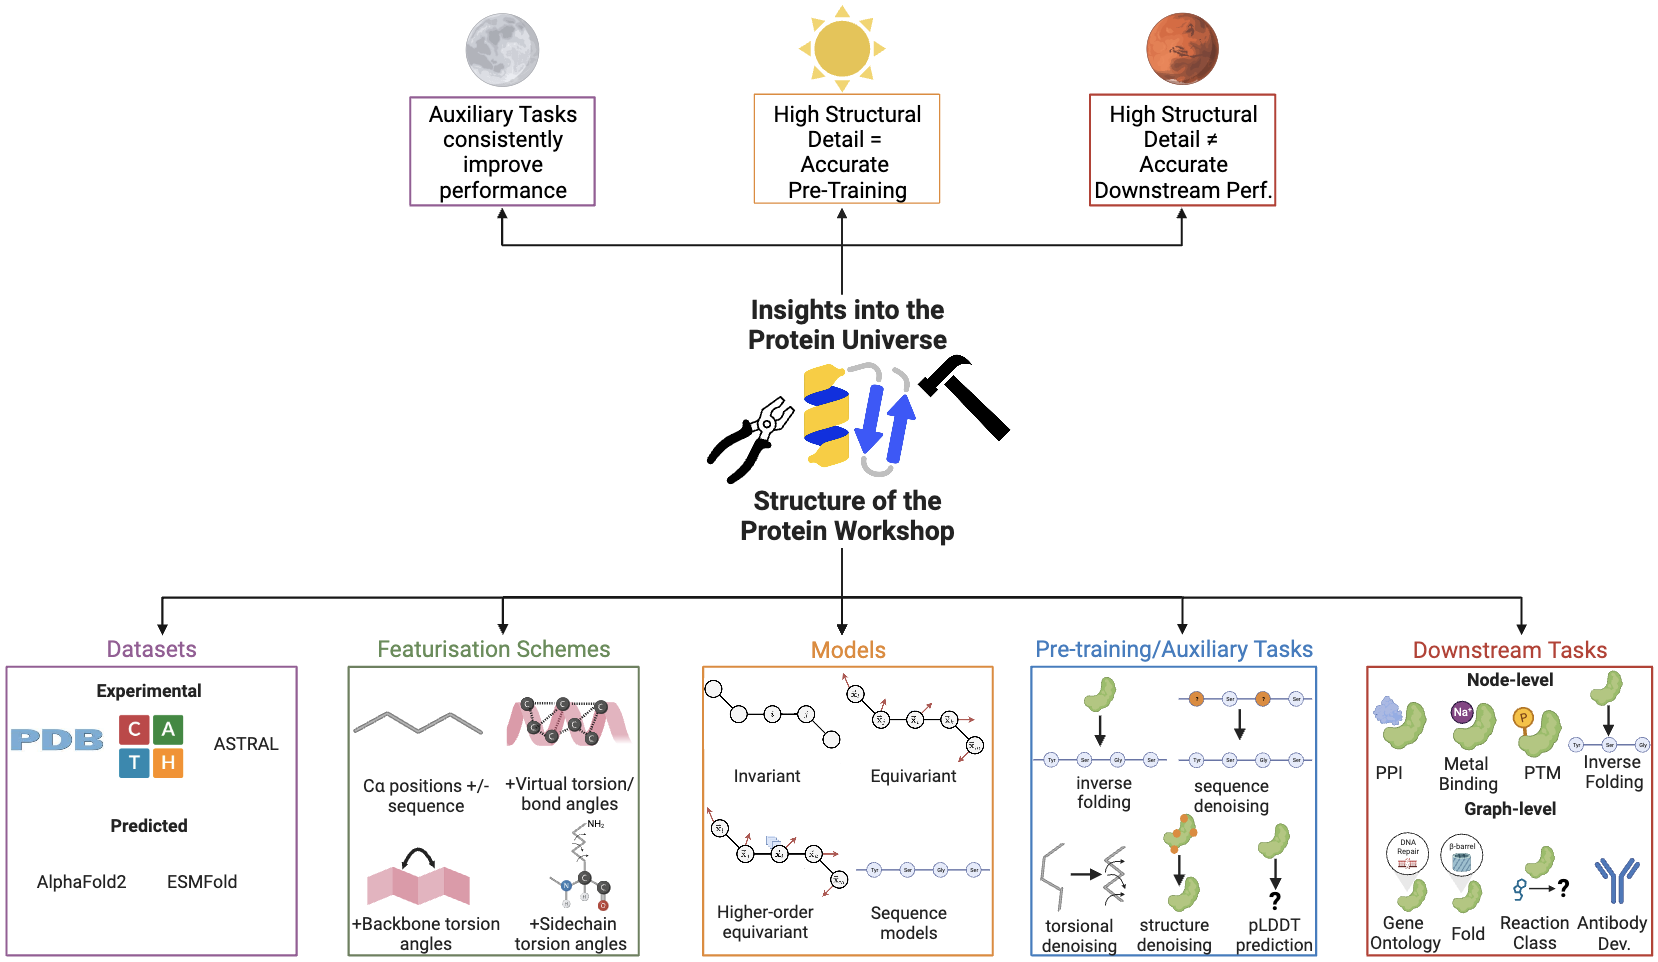
\includegraphics[trim=0 0 0 11.7cm, clip, width=\textwidth]{neurips_data_2023/overview.png}
    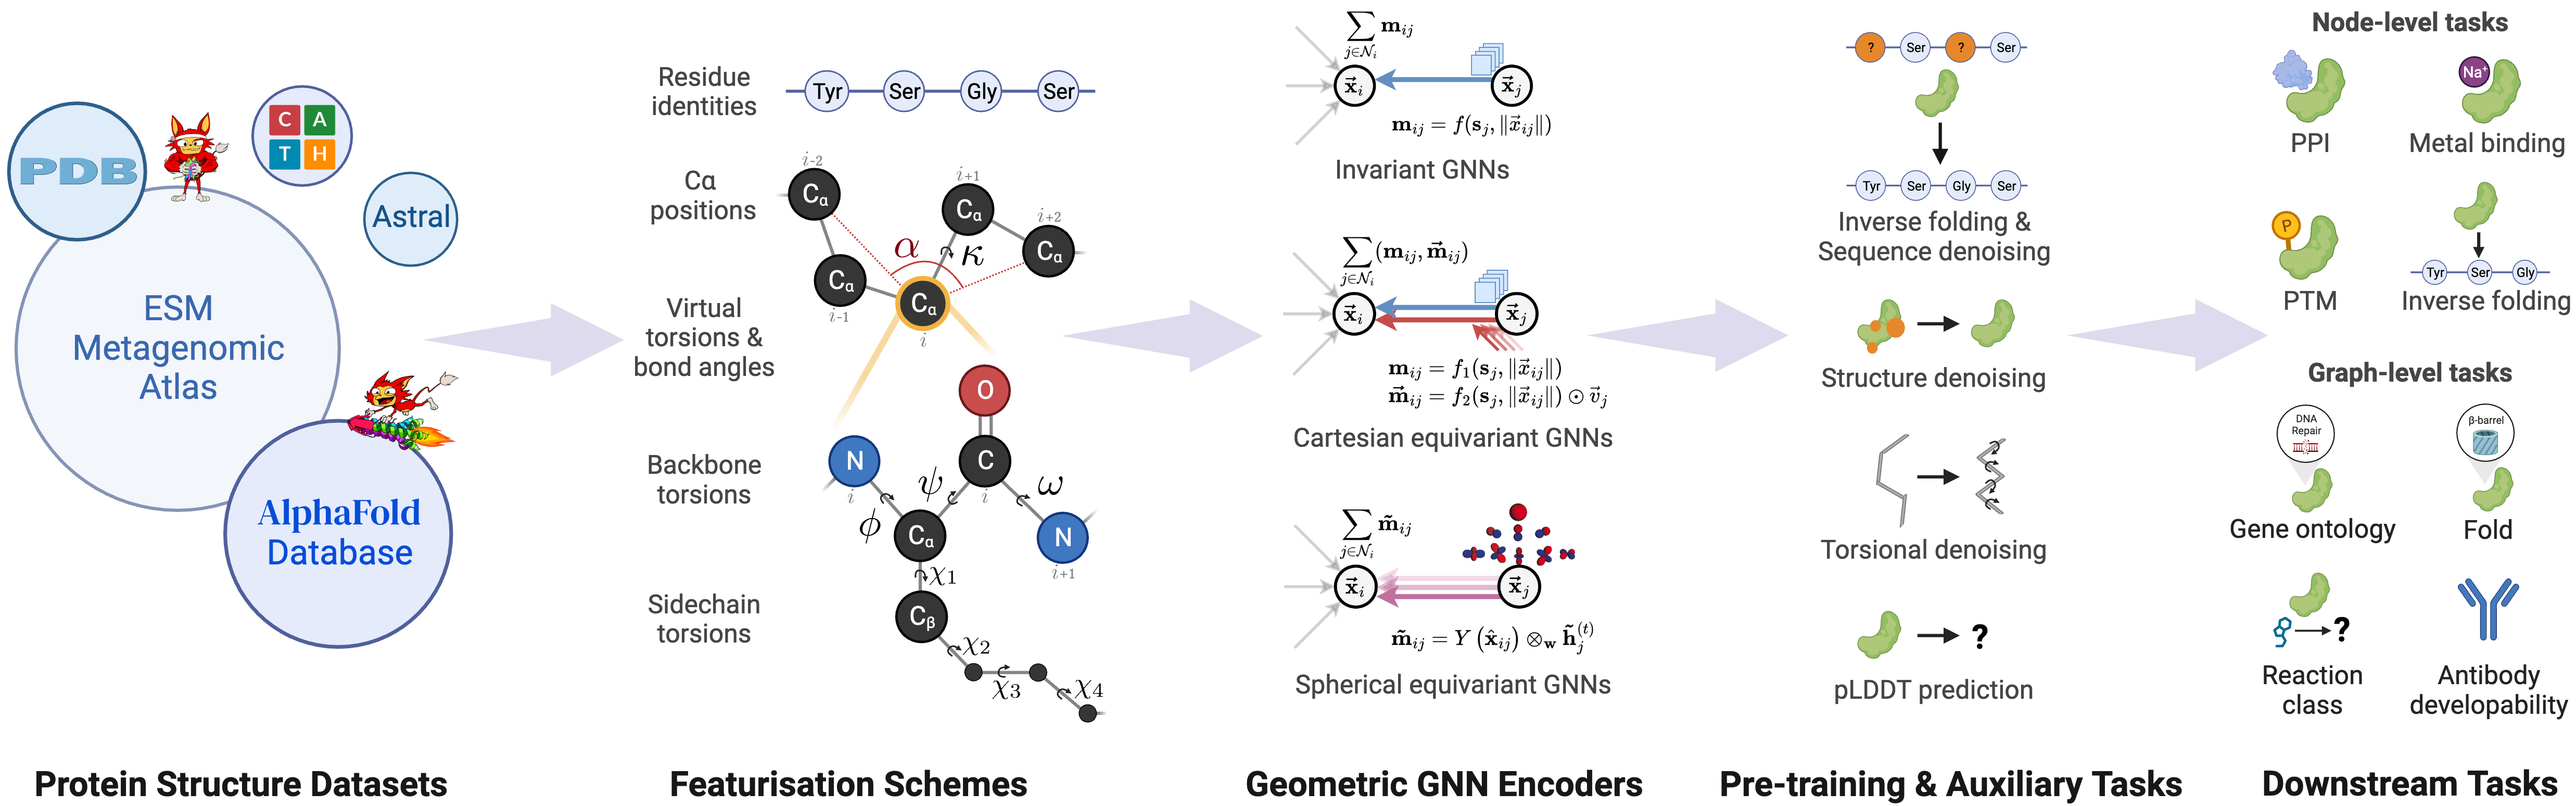
\includegraphics[width=1\textwidth]{iclr_2024/proteinworkshop.jpeg}
    \caption{
    Overview of \emph{ProteinWorkshop}, a comprehensive benchmark suite for evaluating pre-training and representation learning of Geometric GNNs on large-scale protein structure data.
    }
    \label{fig:overview}
\end{figure}

%%%

Our contributions are as follows:\vspace{-5pt}
\begin{itemize}
    \item We curate numerous \emph{structure-based} pretraining and fine-tuning datasets from the literature with a focus on tasks that can enable structural annotation of predicted structures. We compile a highly-modular benchmark, enabling the community to rapidly evaluate protein representation learning methods across tasks, models, and pretraining setups. 
    \item We benchmark Geometric GNNs for representation learning of proteins at different levels of structural granularity (C$\alpha$, backbones, sidechain) and across several classes of models, ranging from general-purpose \citep{schutt2018schnet, satorras2021n} to protein-specific architectures \citep{morehead2024geometry, zhang2023protein}. 
    We are the first to evaluate higher order equivariant GNNs \citep{thomas2018tensor, batatia2022mace} for proteins.
    \item We pretrain and evaluate models on, to our knowledge, the \emph{largest non-redundant} protein structure corpus containing 2.27 million structures from AlphaFoldDB.
    \item Our benchmarks show that sequence denoising-based auxiliary tasks and structure denoising-based pretraining consistently improve Geometric GNNs.
    Moreover, we surprisingly observe that sequence-based pretrained ESM2 \citep{lin2022language} augmented with our structural featurisation matches state-of-the-art GNNs on (super)family fold and gene ontology prediction.
\end{itemize}
% (1) We curate numerous \emph{structure-based} pretraining and fine-tuning datasets from the literature with a focus on tasks that can enable structural annotation of predicted structures. We compile a highly-modular benchmark, enabling the community to rapidly evaluate protein representation learning methods across tasks, models, and pretraining setups. 
% (2) We benchmark protein structure representation learning at different levels of structural granularity (C$\alpha$, backbones, sidechain) and across several families of geometric GNN models, ranging from general-purpose \citep{schutt2018schnet, satorras2021n} to protein-specific architectures \citep{morehead2024geometry, zhang2023protein}. 
% We are the first to evaluate higher order tensor-based equivariant GNNs \citep{thomas2018tensor, batatia2022mace} for protein representation learning.
% (3) We pre-train and evaluate models on, to our knowledge, the \emph{largest non-redundant} protein structure corpus containing 2.27 million structures.
% (4) Our benchmarking study finds that sequence denoising-based auxiliary tasks and structure denoising-based pretraining consistently improve GNN model performance.
% Moreover, we surprisingly observe that sequence-based pretrained ESM2 \citep{lin2022language} augmented with our structural featurisation matches state-of-the-art GNNs on (super)family fold and gene ontology prediction.
% The results of our experiments show, respectively, that sequence denoising-based auxiliary tasks and structure denoising-based pretraining consistently improve the performance of both invariant and equivariant models learning from protein structures. Moreover, we surprisingly observe that sequence-based pretrained models such as ESM2 \citep{lin2022language} provide compelling performance for (super)family fold classification tasks compared to invariant and equivariant GNNs.

\section{Related Work}

\textbf{Protein Structure Representation Learning. } Several structure-based encoders for proteins have been designed to extract information from different levels of granularity, such as residue-level, atom-level and surfaces. Previous works have aimed to encode protein structural priors directly within architectures to model proteins hierarchically \citep{somnath2021multi, hermosilla2020intrinsic}, as computationally efficient point clouds \citep{gainza2020deciphering, sverrisson2021fast}, or as geometric graphs \citep{jing2020learning, jin2021iterative, morehead2024geometry, wang2023learning, zhang2023protein, mahmud2023accurate} for tasks such as protein function prediction \citep{Gligorijevi2021}, protein model quality assessment \citep{eismann2020protein, chen20233d, morehead2024gcpnetema}, and protein interaction region prediction \citep{dai2021protein, morehead2023dips}.

\textbf{Protein Benchmarks. } Several benchmarks have been proposed for evaluating the efficacy of learnt protein \emph{sequence} representations. However, \emph{structure-based} benchmarks are comparatively unaddressed. \citet{tape} developed TAPE (Tasks Assessing Protein Embeddings), providing a large pretraining corpus of protein sequences curated from Pfam \citep{ElGebali2018}, as well as a collection of five supervised benchmark tasks assessing the ability of protein language models to predict structural qualities (contact prediction and secondary structure prediction), and functional properties (fluorescence and stability prediction). \citet{peer} proposed PEER (Protein Sequence Understanding), focussing on multitask evaluation of protein sequence models. Therapeutic Data Commons \citep{NEURIPSDATASETSANDBENCHMARKS2021_4c56ff4c} provide several datasets relevant to therapeutic development, however the few protein structure-derived datasets it contains are cast as sequence-based tasks. \citet{NEURIPSDATASETSANDBENCHMARKS2021_2b44928a} developed FLIP, a sequence-based benchmark of protein fitness landscapes. ProteinGLUE \citep{Capel2022} is another sequenced-based benchmark focussing on per-residue tasks.

To our best knowledge, the only protein structure-benchmark to date is ATOM3D \citep{NEURIPSDATASETSANDBENCHMARKS2021_c45147de}, which proposes a collection of tasks largely assessing geometric methods at predicting graph-level properties of protein structures. TorchProtein \citep{zhu2022torchdrug} also provides a small collection of global-structural datasets. Most existing benchmarks do not exhaustively evaluate both the local and global representation learning power of proposed methods. As the field develops, we identify a need for a consistent benchmarking framework of diverse tasks to ensure improving results reported in the literature map on to progress in the downstream problems we hope to address.
Similar benchmarking efforts for general purpose GNNs have provided experimental rigour to architectural research \citep{dwivedi2020benchmarking}.

\textbf{Denoising-Based Pre-training and Regularisation. } 
Several methods have been developed for pre-training GNNs, predominantly focussing on cases where 3D coordinate information is only implicitly encoded in the graph structures. In this work, we build on work by \citet{godwin2021simple} and \citet{zaidi2023pretraining} to investigate whether denoising-based auxillary and pre-training tasks are effective methods for pre-training geometric GNNs operating on protein structures, similar to concurrent works bridging the gap between denoising objectives for geometric neural networks and diffusion generative modeling for biomolecules \citep{huang2023data, corso2023modeling}.
\section{ProteinWorkshop}
The overarching goal of \emph{ProteinWorkshop} is to effectively cover the design space of protein structure representation learning methods. To achieve this, the benchmark is highly modular by design, enabling evaluation of different combinations of structural encoders, protein featurisation schemes, and auxiliary tasks over a wide range of both supervised and unsupervised tasks.
A user manual is available in Appendix \ref{app:benchmark}, containing detailed listings and descriptions of all components.

\subsection{Featurisation Schemes}
Protein structures are typically represented as geometric graphs, with researchers opting to use a coarse-grained C$\alpha$ atoms graph as full atom representations can quickly become computationally intractable due to a large number of nodes. 
However, this is a lossy representation, with much of the structural detail, such as orientation of the backbone and sidechain structure, being only implicitly encoded.
Due to the computational burden incurred by operating on full-atom node representations, we focus primarily on C$\alpha$-based graph representations, investigating featurisation strategies to incorporate higher-level structural information. 
Note that we do provide utilities to enable users to work with backbone and full-atom graphs in the benchmark.
% We represent protein structures as geometric graphs, $\mathcal{G} = (\mathcal{V}, \mathcal{E}, \mathbf{\vec{X}}, \mathbf{S}, \mathbf{\vec{V}})$, where $\mathcal{V}$ is a set of nodes, $\mathcal{E}$ is a set of edges, $\mathbf{\vec{X}} \in \mathbb{R}^{|\mathcal{V}| \times 3}$ is a matrix of Cartesian node coordinates, $\mathbf{S} \in \mathbb{R}^{|\mathcal{V}| \times d}$ is a matrix of $d$-dimension scalar node features, and $\mathbf{\vec{V}} \in \mathbb{R}^{|\mathcal{V}| \times d \times 3}$ is a tensor of vector-valued features. 
Details about different featurisation schemes are provided in Appendix \ref{app:featurisation} and Table \ref{tab:features}.

\subsection{Pre-training Tasks}

The benchmark contains a comprehensive suite of pretraining tasks. Broadly, these can be categorised into: masked-attribute prediction, denoising-based and contrastive learning-based tasks. These can be used as both a pretraining objective or as auxiliary tasks in a downstream supervised task.

\textbf{Sequence Denoising. } The benchmark contains two variations based on two sequence corruption processes $C(\tilde{\mathcal{S}} | \mathcal{S}, \nu)$ that receive an amino acid sequence $\mathcal{S} \in [0, 1]^{|\mathcal{V}| \times 23 }$ and return a sequence $\mathcal{S} \in [0, 1]^{|\mathcal{V}| \times 23 }$ with fraction $\nu$ of its positions corrupted. The first scheme is based on mutating a fraction of the residues to a random amino acid and tasking the model with recovering the uncorrupted sequence. The second is a masked residue prediction task, where a fraction of the residues are altered to a mask value and the model is tasked to recover the uncorrupted sequence.

\textbf{Structure Denoising. } We provide two structure-based denoising tasks: coordinate denoising and torsional denoising. In the coordinate denoising task, noise is sampled from a normal or uniform distribution and scaled by noise factor, $\nu \in \mathbb{R}$, and applied to each of the atom coordinates in the structure to ensure structural features, such as backbone or sidechain torsion angles, are also corrupted. The model is then tasked with predicting either the per-node noise or the original uncorrupted coordinates. For torsional denoising, the noise is applied to the backbone torsion angles and Cartesian coordinates are recomputed using pNeRF \citep{AlQuraishi2019} and the uncorrupted bond lengths and angles prior to feature computation. Similarly to the coordinate denoising task, the model is then tasked with predicting either the per-residue angular noise or the original dihedral angles.

\textbf{Sequence-Structure Co-Denoising. } This is a multitask formulation of the previously described structure and sequence denoising tasks, with separate output heads for denoising each modality.

\textbf{Masked Attribute Prediction. } 
We use inverse folding (Section \ref{sec:inverse-folding}) as a pretraining task.
The benchmark additionally incorporates the distance, angle and dihedral angle masked-attribute prediction \citep{zhang2023protein} as well as a backbone dihedral angle prediction task.

\textbf{pLDDT Prediction. } Structure prediction models typically provide per-residue pLDDT (predicted Local Distance Difference Test) scores as local confidence measures which have been shown to correlate well with disordered regions \citep{wilson2022alphafold2}. We formulate a node-level regression task on predicted structures, somewhat analogous to structure quality assessment, where the model is tasked with predicting the scaled per-residue pLDDT $y \in [0, 1]$ values.

%%%

\subsection{Downstream Tasks}
We curate several structure-based and sequence-based datasets from the literature and existing benchmarks\footnote{To retain focus on \emph{protein} representation learning, we deliberately exclude commonly-used tasks based on protein-small molecule interactions as it is hard to disentangle the effect of the small molecule representation and the potential for bias \citep{Boyles2019}}, summarised in Table \ref{tab:datasets}. The tasks are selected to evaluate not only the \emph{global} structure representational power of each method, but also to evaluate the ability of each method to learn informative \emph{local} representations for residue-level prediction and annotation tasks.

The raw structures are, where possible and accounting for obsolescence, retrieved directly from the PDB (or another structural source) as several processed datasets used by the community discard full atomic coordinates in favour of retaining only $C_\alpha$ positions, making them unsuitable for in-depth experimentation. 
This provides an entry point for users to apply a custom sequence of pre-processing steps, such as deprotonation or fixing missing regions which are common in experimental data.

\begin{table*}[!t]
    \centering
    \caption{\textbf{Overview of supervised tasks and datasets.}}
    \begin{adjustbox}{max width=\linewidth}
        \begin{tabular}{llcccccc}
        \toprule
        & \textbf{Task} & \textbf{Dataset Origin} & \textbf{Structures} &  \textbf{\# Train} & \textbf{\# Validation} & \textbf{\# Test} & \textbf{Metric} \\
        \midrule
        \multirow{4}{*}{\rotatebox[origin=c]{90}{Node-level}} &
        Inverse Folding & \citet{NEURIPS2019_f3a4ff48} & Experimental
        &
        3.9 M
        &
        105 K
        & 
        180 K & Perplexity
        \\
        & PPI Site Prediction & \citet{gainza2020deciphering} & Experimental 
        &
        478 K
        & 
        53 K
        &
        117 K & AUPRC
        \\
        & Metal Binding Site Prediction & & Experimental
        &
        1.1 M
        &
        13.7 K
        &
        29.8 K & Accuracy
        \\
        & Post-Trans. Mod. Site Prediction &
        \citet{Yan2023} & Predicted 
        
        &
        44 K
        &
        2.4 K
        &
        2.5 K & ROC-AUC \\
        \midrule
        \multirow{4}{*}{\rotatebox[origin=c]{90}{Graph-level}}
        & Fold Prediction & \citet{hou2017} & Experimental 
        &
        12.3 K
        &
        0.7 K
        &
        1.3/0.7/1.3 K & Accuracy
        \\
        & Gene Ontology Prediction & \citet{Gligorijevi2021} & Experimental 
        &
        27.5 K
        &
        3.1 K
        &
        3.0 K & F$_{\text{max}}$
        \\
        & Reaction Class Prediction & \citet{hermosilla2020intrinsic} &  Experimental 
        &
        29.2 K
        &
        2.6 K
        &
        5.6 K & Accuracy
        \\
        & Antibody Dev. Prediction & \citet{NEURIPSDATASETSANDBENCHMARKS2021_4c56ff4c} & Experimental 
        &
        1.7 K
        &
        0.24 K
        &
        0.48 K & AUPRC
        \\
        \bottomrule
        \end{tabular}
    \end{adjustbox}
    \label{tab:datasets}
\end{table*}

%%%

\subsubsection{Node-level Tasks}

\textbf{Inverse Folding. }
\label{sec:inverse-folding} 
Many generative methods for protein design produce backbone structures that require the design of an associated sequence. As a result, inverse folding is an important part of \emph{de novo} design pipelines for proteins \citep{Dauparas2022}.
% This task is a common protein engineering task where the goal is to recover an amino acid sequence given a structure up to backbone completeness. 
Formally, this is a node-level classification task where the model learns a mapping for each residue $r_i$ to an amino acid type $y \in \{1, \dots, n \}$, where $n$ is the vocabulary size ($n=20$ for the canonical set of amino acids).
Inverse folding is a generic task that can be applied to any dataset in the benchmark. In the literature, it is commonly evaluated on the CATH dataset (Section \ref{sec:pre-train-data}) compiled by \citet{NEURIPS2019_f3a4ff48}.

\textbf{PPI Site Prediction. } 
Identifying protein-protein interaction sites has important applications in developing refined protein-protein interaction networks and docking tools, providing biological context to guide protein engineering and target identification in drug discovery campaigns \citep{Jamasb2021}.
This task is a node-level binary classification task where the goal is to predict whether or not a residue is involved in a protein-protein interaction interface.
We use the dataset of experimental structures curated from the PDB by \citet{gainza2020deciphering} and retain the original splits, though we modify the labelling scheme to be based on inter-atomic proximity (3.5 \AA), which can be user-defined, rather than solvent exclusion. The dataset is curated from the PDB by preprocessing such as the presence of one of the seven specified ligands (e.g., ADP or FAD), clustering based on 30\% sequence identity and random subsampling. It contains 1,459 structures, which are randomly assigned to training (72\%), validation (8\%) and test set (20\%). 12 (\AA) radius patches were extracted from the generated structures and a patch labelled as part of a binding pocket if its centre point was < 3 (\AA) away from an atom of the corresponding ligand.

\textbf{Metal Binding Site Prediction. } 
Many proteins coordinate transition metal ions to carry out their functions. Predicting the binding sites of metal ions can elucidate the role of metal binding on protein function.
This is a binary node classification task where each residue is mapped to a label $y \in \{0, 1\}$ indicating whether the residue (or its constituent atoms) is within 3.5 (\AA) of a user-defined metal ion or ligand heteroatom, respectively.
We provide tooling to curate a dataset of experimental structures from the PDB for this task, where binding site assignments for each residue are computed on-the-fly. While the benchmark supports this task on arbitrary subsets of the PDB and ligands, we provide the Zinc-binding dataset from \citet{Drr2023} specifically for this task. The dataset is constructed by sequence-based clustering of the PDB at 30\% sequence identity to remove sequence and structural redundancy. Clusters with a member shorter than 3000 residues, containing at least one zinc atom with resolution better than 2.5 (\AA) determined by x-ray crystallography and not containing nucleic acids are used to compose the dataset. If multiple structures fulfil these criteria, the highest resolution structure is used. The train (2,085) / validation (26) / test (59) splits are constructed such that proteins in the validation and test sets have no partial overlap with any protein in the training data.


\textbf{Post-Translational Modification Site Prediction. } 
Identifying the precise sites where post-translational modifications (PTMs) occur is essential for understanding protein behaviour and designing targeted therapeutic interventions.
We frame prediction of PTM sites as a multilabel classification task where each residue is mapped to a label $y \in \{1, \dots, 13\}$ distinguishing between modifications on different amino acids (e.g. phosphorylation on S/T/Y and N-linked glycosylation on N).
We use a dataset of 48,811 AlphaFold2-predicted structures curated by \citet{Yan2023}, where each structure contains the PTM metadata necessary to construct residue-wise site prediction labels. The dataset is split into training (43,907, validation (2,393) and test (2,511) sets based on 50\% sequence identity and 80\% coverage.

\subsubsection{Graph-level Tasks}

\textbf{Fold Prediction. }
The utility of this task is that it serves as a litmus test for the ability of a model to distinguish different structural folds. It stands to reason that models that perform poorly on distinguishing fold classes likely learn limited or low-quality structural representations.
This is a multiclass graph classification task where each protein, $\mathcal{G}$, is mapped to a label $y \in \{1, \dots, 1195\}$ denoting the fold class.
We adopt the fold classification dataset originally curated from SCOP 1.75 by \citep{hou2017}. This provides three different test sets stratified based on topological similarity: Fold, in which proteins originating from the same superfamily are absent during training; Superfamily, in which proteins originating from the same family are absent during training; and Family, in which proteins from the same family are present during training.

\textbf{Gene Ontology Prediction. }
Predicting protein function in the form of functional annotations such as GO terms has important applications in protein analysis and engineering, providing researchers with the ability to cluster functionally-related structures or to guide protein generation methods to design new proteins with desired functional properties.
This is a multilabel classification task, assigning functional Gene Ontology (GO) annotation to structures. GO annotations are assigned within three ontologies: biological process (BP), cellular component (CC) and molecular function (MF). We use the dataset of experimental structures curated from the PDB by \citet{Gligorijevi2021} and retain the original multi-cutoff based splits, with cutoff at 95\% sequence similarity. 

\textbf{Reaction Class Prediction. } 
As proteins' reaction classifications are based on their enzyme-catalyzed reaction according to all four levels of the standard Enzyme Commission (EC) number, methods that predict such classifications may help elucidate the function of newly-designed proteins as they are developed.
This is a multiclass graph classification task where each protein, $\mathcal{G}$, is mapped to a label $y \in {\{1, ..., 384\}}$ denoting which class of reactions a given protein catalyzes; all four levels of the EC assignment are employed to define the reaction class label.
We adopt the reaction class prediction dataset originally curated from the PDB by \citet{hermosilla2020intrinsic}, split on the basis of sequence similarity using a 50\% threshold.

\textbf{Antibody Developability Prediction. }
Therapeutic antibodies must be optimised for favourable physicochemical properties in addition to target binding affinity and specificity to be viable development candidates. Consequently, we frame prediction of antibody developability as a binary graph classification task indicating whether a given antibody is developable.We adopt the antibody developability dataset originally curated from SabDab \citep{dunbar2014sabdab} by \citet{Chen2020}.
This dataset contains 2,426 antibodies that have both sequences and PDB structures available, where each example contains both a heavy chain and a light chain with resolution < 3 (\AA). 
The label is based on thresholding the developability index (DI) \citep{Lauer2012} 
as computed by BIOVIA's platform \citep{Accelrys2018BioviaDiscoveryStudio}, which relies on an antibody's hydrophobic and electrostatic interactions.
This task is interesting from a benchmarking perspective as it enables targeted performance assessment of models on a specific (immunoglobulin) fold, providing insight into whether general-purpose structure-based encoders can be applicable to fold-specific tasks.

\subsection{Pre-training Datasets}\label{sec:pre-train-data}

The benchmark contains several large corpora of both experimental and predicted structures that can be used for pretraining or inference. We provide utilities for configuring supervised tasks and splits directly from the PDB.
Additionally, we build storage-efficient dataloaders for large pretraining corpora of predicted structures (AlphaFoldDB, ESM Atlas).
We believe our codebase will considerably reduce the barrier to entry for working with large structure-based datasets. 
% Additionally, we provide ready-to-go dataloaders for several large-scale collections of predicted structures derived from both AlphaFold2 \citep{jumper2021highly} and ESMFold \citep{lin2022language}. 
% This is facilitated by FoldComp \citep{Kim2023}, a (minimally) lossy compression scheme for predicted protein structures. FoldComp stores protein structures as a collection of discretised dihedral and bond angles which can be used to reconstruct the whole structure using fixed bond lengths and canonical amino acid geometry. FoldComp achieves a disk-space reduction of almost an order of magnitude, describing a residue with only 13 bytes -- down from 97 bytes per-residue in a traditional uncompressed format. Whilst lossy, this procedure results in 0.08 \AA\ and 0.14 \AA\ RMSD for backbone and all-atom reconstruction, making it highly suitable for pretraining tasks which use input representations complete up to the backbone. Furthermore, this lightweight format enables the dataloaders in the benchmark to read structures \emph{directly from disk} with no pre-processing or caching required.

\subsubsection{Experimental Structures}

\textbf{PDB. } We provide utilities for curating datasets directly from the Protein Data Bank \citep{Berman2000}. In addition to using the collection in its entirety, users can define filters to subset and split the data using a combination of structural similarity, sequence similarity or temporal strategies. Structures can be filtered by length, number of chains, resolution, deposition date, presence/absence of particular ligands and structure determination method. 
% The benchmark supports working with PDB structures in both \texttt{.pdb} and \texttt{.mmtf} format \citep{Bradley2017}, which significantly reduces the requirements for data storage.

\textbf{CATH. } We provide the dataset derived from CATH 4.2 40\% \citep{Knudsen2010} non-redundant chains developed by \citet{NEURIPS2019_f3a4ff48} as an additional, smaller, pretraining dataset. 
% These data are split based on random assignment of the CATH topology classifications based on an 80/10/10 split.

\textbf{ASTRAL. } ASTRAL \citep{Brenner2000} provides protein \emph{domain} structures which are regions of proteins that can maintain their structure and function independently of the rest of the protein. Domains typically exhibit highly-specific functions and can be considered structural building blocks.

\subsubsection{Predicted Structures}

\textbf{AlphaFoldDB Representative Structures.} This dataset contains 2.27 million representative structures, identified through large-scale structural-similarity-based clustering of the 214 million structures contained in the AlphaFold Database \citep{Varadi2021} using FoldSeek \citep{vanKempen2023}. We additionally provide a subset of this collection --- the so-called dark proteome --- corresponding to the 31\% of the representative structures that lack annotations.

\textbf{ESM Atlas, ESM High Quality.} These datasets are compressed collections of predicted structures produced by ESMFold. ESM Atlas is the full collection of all 772m predicted structures for the MGnify 2023 release \citep{Richardson2022}. ESM High Quality is a curated subset of high confidence (mean pLDDT) structures from the collection.

\section{Methods and Experimental Setup}

\textbf{Overview. }
To demonstrate the utility of our benchmark, we investigate how combinations of protein structure representation, architecture choice and pretraining/auxiliary tasks affect predictive performance across a range of tasks. The tasks are selected to focus on important real-world structural annotation tasks and such that we can evaluate these combinations in terms of both the local and global representational power. To this end, we select state-of-the-art protein structure encoders and generic geometric GNN architectures that span the design space of geometric GNN models with regard to both message passing body order and tensor order \citep{joshi2023expressive}. 
We evaluate several structural representations that, to varying degrees, capture the full detail of the protein structure.

\textbf{Architectures. }
% To investigate the effectiveness of geometric graph neural networks, we provide a unified implementation of several rotationally invariant and equivariant architectures spanning the range of message passing body order and tensor order \citep{joshi2023expressive}, including general-purpose as well as protein-specific models. Implementation details and hyperparameters are provided in the Appendix. Note, for our ESM sequence baseline, * denotes results taken from \citet{zhang2023protein}.
We provide a unified implementation of several rotation invariant and equivariant architectures. 
We benchmark 4 general purpose models: SchNet \citep{schutt2018schnet}, EGNN \citep{satorras2021n}, TFN \citep{thomas2018tensor}, MACE \citep{batatia2022mace}; and 2 protein-specific architectures: GCPNet \citep{morehead2024geometry}, GearNet \citep{zhang2023protein}.
% See Appendix \ref{app:gnns} for detailed equations and hyperparameters.
We also compare geometric GNNs to the pretrained sequence-based language model ESM \citep{lin2022language} augmented with structural featurisation.
We chose the 650M pretrained ESM2 because this is the scale at which significant structure-related abilities were observed for ESM.
% Our results further reinforce their observation – we find that combining ESM2 650M with our structural featurisation yields extremely strong results on Fold classification tasks.

\textbf{Featurisation Schemes. } We consider five featurisation schemes, progressively increasing the amount of structural information provided to the model by incorporating sequence positional information, virtual dihedral and bond angles over the
\caa 
trace, backbone torsion angles, and sidechain torsion angles. Featurisation schemes are detailed in Table \ref{tab:features} in the Appendix.

\textbf{Pretraining Dataset. } For all pretraining experiments we use AlphaFoldDB \citep{BarrioHernandez2023}. 
This dataset provides a rich diversity of 2.27 million non-redundant protein structures and, to our knowledge, is substantially more diverse than any other previously used structure-based pretraining corpus, whilst remaining of a size that is amenable to experimentation.
Models pretrained on AlphaFoldDB should, in principle, exhibit strong generalisation to the currently known (and predicted) natural protein structure universe as it would have `seen'
 the same protein fold during pretraining.
To facilitate working with large-scale AlphaFoldDB and ESMAtlas, we developed storage-efficient dataloaders based on FoldComp \citet{Kim2023}, described in Appendix \ref{app:pretrain-data}.

\textbf{Pretraining and Auxiliary Tasks. } In our evaluation, we focus predominantly on denoising-based pretraining and auxiliary tasks as these are comparatively less explored than contrastive or masked-attribute prediction tasks \citep{zhang2023protein}. We consider five pretraining tasks: (1) structure-based denoising, (2) sequence denoising, (3) torsional denoising, (4) inverse folding and (5) pLDDT prediction. Structure and sequence denoising are also used as auxiliary tasks in our experiments.
We also investigate an inverse folding pre-training task which we subsequently finetune on the CATH dataset for benchmarking inverse folding as a downstream task (see below).
% The benchmark supports several additional pretraining tasks detailed in Appendix \ref{app:pretraining-tasks}.

\textbf{Noising Schemes. } For structure-based denoising we draw i.i.d. noise samples from a Gaussian distribution and scale by $\sigma=0.1$ to corrupt the input coordinates or dihedral angles. Geometric scalar and vector-valued features are computed from the noised structure, \textit{i.e.}
$\tilde{\mathcal{G}} = (\mathcal{V}, \tilde{\mathcal{E}}, \tilde{\mathbf{X}}, \tilde{\mathbf{S}}, \tilde{\mathbf{V}}), \mathrm{ where }\ \tilde{\vx_{i}} = \vx_{i} + \sigma \bm{\epsilon}_{i}\ \mathrm{ and }\ \bm{\epsilon}_{i} \sim \mathcal{N}(0, I_3).
$
For sequence-based denoising, we use the mutation strategy and corrupt 25\% of the residues in each protein. When sequence denoising is used as an auxiliary task, we weight the loss with a coefficient $\lambda = 0.1$, similar to NoisyNodes \citep{godwin2021simple}. 

% \hl{
% \textbf{Downstream Tasks. } Due to the large hardware requirements of our initial benchmark, we currently evaluate on two representative structure-based tasks, \textbf{fold classification} (to evaluate methods' global protein representations) and \textbf{inverse folding} (to evaluate methods' local protein representations), whereas six other tasks are available in our proposed benchmark. 
% }
% Appendix \ref{app:datasheets} contains detailed documentation for all 8 downstream tasks available in our benchmark. 
% To address this limitation, in the near future, we plan to add supplementary experiments covering more of such tasks in our benchmark results.

\textbf{Training. }
As we are interested in benchmarking large-scale datasets and models, we try to consistently use six layers for all models, each with 512 hidden channels. For equivariant GNNs, we reduced the number of layers and hidden channels to fit 80GB of GPU memory on one NVIDIA A100 GPU.
For downstream tasks, we set the maximum number of epochs to 150 and use the Adam optimizer with a batch size of 32 and ReduceLROnPlateau learning rate scheduler, monitoring the validation metric with patience of 5 epochs and reduction of 0.6. 
See Appendix \ref{app:hyperparameters} for details on hyperparameter tuning for optimal learning rates and dropouts for each architecture.
We train models to convergence, monitoring the validation metric and performing early stopping with a patience of 10 epochs.
Pretraining is performed for 10 epochs using a linear warm-up with cosine schedule. 
We report standard deviations over three runs across three random seeds.
\section{Results \& Discussions}

\subsection{Auxiliary Sequence Denoising Consistently Improves Baseline Performance}

In Table \ref{tab:baseline_graph_classification_results}, we first set out to determine the following questions about architectural choices in conjunction with denoising auxiliary tasks and \textit{without} pretraining:
\begin{enumerate}
    \item \textbf{Whether invariant or equivariant models perform better?} Across 8 tasks, equivariant models such as EGNN, GCPNet and TFN attain the best performance on 5.
    Notably, sequence-based ESM augmented with our structural featurisation matches state-of-the-art protein-specific GNNs \citep{fan2023continuousdiscrete} on (super)family and gene ontology prediction.
    \item \textbf{Which input representation is the best for each respective task?} Featurising models with \caa atoms, virtual angles, and backbone torsions provides the best performance overall on 21 out of 48 combinations of models and tasks. This suggests that letting models implicitly learn about side chain orientation and flexibility by using backbone-only featurisation may prevent overfitting on crystallisation artifacts \citep{Dauparas2022}.
    \item \textbf{Whether auxiliary denoising tasks improve model performance?} Sequence denoising is a particularly useful auxiliary task for training protein structure encoders until sufficient structural detail makes the task trivial, improving results over not using auxiliary tasks for 98 out of 210 combinations of models, task, and auxiliary tasks.
    Notably, structure denoising helped stabilise the training of MACE models on the GO-CC and Reaction tasks, where other runs did not converge.
\end{enumerate}

% We first set out to determine (1) whether invariant or equivariant models perform better on our set of tasks, (2) which input representation is the best for each respective task and (3) whether auxiliary denoising tasks improve model performance. Table \ref{tab:baseline_graph_classification_results} shows that (1) equivariant models such as EGNN and GCPNet produce the best global and local representations for fold classification and inverse folding, respectively, whereas sequence-based models (i.e., ESM) produce the best representations for (super)family classification. (2) Notably, featurising models with C$\alpha$ atoms and virtual angles provide the best performance overall. The same set of results also suggests that (3) sequence denoising is a particularly useful auxiliary task for training protein structure encoders.

\subsection{Incorporating More Structural Detail Improves Pre-Training Performance}

We then investigated protein structure pre-training in Table  \ref{tab:pre-training} to find out:
\begin{enumerate}
    \item \textbf{Which input representation is best for pre-training?} Incorporating dihedral angles consistently improves validation metrics on pre-training tasks, more so than architecture.
    \item \textbf{Which GNNs benefit from which pre-training task?} Inverse folding, sequence denoising, and torsional denoising benefit equivariant models the most in the context of pre-training, whereas pLDDT prediction and structure denoising benefit invariant models the most, suggesting that certain pre-training tasks benefit certain classes of models more than other tasks.
    Unfortunately, we were currently unable to pre-train spherical equivariant GNNs (TFN, MACE) due to the high computational requirements of these models.
\end{enumerate}

% We then investigated protein structure pre-training to find out (1) which input representation is best for pre-training and (2) which geometric neural networks benefit from which pre-training task. Table \ref{tab:pre-training} shows that (1) incorporating dihedral angles consistently improves validation metrics on pre-training tasks, more so than architecture. These results also suggest that (2) inverse folding, sequence denoising, and torsional denoising benefit equivariant models the most in the context of pre-training, whereas pLDDT prediction and structure denoising benefit invariant models the most, suggesting that certain pre-training tasks benefit certain classes of models more than other tasks.

%%%

\begin{landscape}

\begin{table}[!t]

\caption{
\textbf{Baseline benchmark results without pretraining.} Results for each model and featurisation pair are given as: \colorbox{orange!20}{no auxiliary task} / \colorbox{blue!20}{+sequence denoising} / \colorbox{green!20}{+structure denoising}. Coloured boxes mark the best auxiliary tasks per model and featurisation, \underline{underlined results} denote the best featurisation choice per model, and \textbf{bold results} are the best models for each task. 
\colorbox{gray!20}{Greyed} cells denote invalid task-setup combinations (e.g. inverse folding and sequence denoising as auxiliary task), and ----- denote runs that did not converge. 
[*] denotes results for ESM without structural features, taken from \citet{zhang2023protein}.
\textbf{Key takeaways:} (1) Sequence denoising as an auxiliary task consistently improves performance across models.
(2) Equivariant GNNs outperform invariant GNNs, in general.
(3) \caa, virtual angles, and backbone torsions provide the best featurisation.
(4) Augmenting ESM2 with structural features provides compelling performance for (super)family fold classification and gene ontology prediction compared to GNNs.
% Baseline tasks without pre-training. Results are given as: \colorbox{orange!20}{no auxiliary task} / \colorbox{blue!20}{+sequence denoising} / \colorbox{green!20}{+structure denoising}. Coloured boxes mark the best auxiliary tasks per method and featurisation, underline the best featurisation per method and bold the best method, all on a per-task basis. Greyed cells denote invalid task-setup combinations (e.g. inverse folding and sequence denoising as auxiliary task). Sequence denoising consistently improves performance. %Lines denote configurations that failed to converge after 6 hours.} 
}
\label{tab:baseline_graph_classification_results}

\begin{adjustbox}{max width=\linewidth}
\begin{tabular}{lllcccccccccccccl}
\toprule
\multirow{2}{*}{\textbf{Method}} & \multicolumn{1}{c}{\multirow{2}{*}{\textbf{Features}}} &%\multicolumn{1}{c}{\multirow{2}{*}{\textbf{EC} ($\uparrow$)}} 
\multicolumn{3}{c}{\multirow{2}{*}{\textbf{GO-CC} ($\uparrow$)}} & \multirow{2}{*}{\textbf{Ab. Dev.} ($\uparrow$)} & \multicolumn{3}{c}{\textbf{Fold} ($\uparrow$)} & \multirow{2}{*}{\textbf{Reaction} ($\uparrow$)} & \multirow{2}{*}{\textbf{PPI} ($\uparrow$)} &
%\multirow{2}{*}{\textbf{PTM} ($\uparrow$)} 
%& \multirow{2}{*}{\textbf{PTM} ($\downarrow$)} & 
& &
\multirow{2}{*}{\textbf{Inverse Folding} ($\downarrow$)}\\
% \cmidrule{3-5}
\cmidrule{7-9}
 %& \multicolumn{1}{c}{} & \textbf{BP} & \textbf{MF} 
 & & &
 & & \multicolumn{1}{c}{} & \textbf{Fold} & \textbf{Family} & \textbf{Superfamily} &  &  &  &  &  &  &  &   \\
\midrule 


\multirow{2}{*}{ESM} & Seq. & & & 0.394* & 0.91 & 26.8* & 97.8* & 60.1* & 80.87 & 0.953 & & & N/A\\ 
&  + \virt, \bb &  & & \textbf{0.545$\pm 0.00$}
& 0.91 & 39.89$\pm 0.00$  & \textbf{99.69}$\pm 0.00$ & \textbf{78.68}$\pm 0.00$  & 81.79 & 0.953$\pm0.00$ &  &  & N/A &  &  &  \\


\midrule 

\multirow{5}{*}{SchNet} & \caa &  & 
%49.70 / \colorbox{blue!20}{57.45} / 44.50 
& 0.387$\pm 0.01$ / 0.415$\pm 0.00$ / \colorbox{green!20}{0.418$\pm 0.00$} & \colorbox{orange!20}{0.89$\pm 0.00$} / 0.88$\pm 0.00$ / 0.82$\pm 0.00$ & 27.11$\pm 0.01$ /  \colorbox{blue!20}{31.36$\pm 0.01$} / 26.05$\pm 0.01$& 81.29$\pm 0.02$ / \colorbox{blue!20}{84.88$\pm 0.01$} / 79.03$\pm 0.03$& 30.02$\pm 0.00$  / \colorbox{blue!20}{34.79$\pm 0.01$} / 27.79$\pm 0.01$& 58.94$\pm 0.01$ / \colorbox{blue!20}{68.33$\pm 0.01$} / 57.59$\pm 0.03$ & 0.954$\pm 0.00$ / 0.952$\pm 0.00$ / \colorbox{green!20}{0.955$\pm 0.00$} & &  & \cellcolor{gray!20} &  &  &  \\

 & + Seq. &  & 
 %46.44 / \colorbox{blue!20}{53.83} / 45.25 
 & 0.390$\pm 0.00$ / 0.374$\pm 0.03$ / \colorbox{green!20}{0.421$\pm 0.00$} & 0.85$\pm 0.05$ / 0.86 / \colorbox{green!20}{0.87} & 34.44$\pm 0.00$ / \colorbox{blue!20}{\underline{38.06$\pm 0.01$}} / 33.31$\pm 0.01$& 91.12$\pm 0.02$ / \colorbox{blue!20}{92.59$\pm 0.01$} / 91.82$\pm 0.02$&  39.33$\pm0.02$ / \colorbox{blue!20}{44.27$\pm 0.01$} / 39.67$\pm 0.01$& \colorbox{orange!20}{70.30$\pm 0.01$} / 68.83$\pm 0.01$ / 62.94$\pm 0.10$ & \colorbox{orange!20}{0.953$\pm 0.00$} / 0.950$\pm 0.00$ / 0.953$\pm 0.00$ & & & \colorbox{orange!20}{11.78$\pm 0.08$} /  12.34$\pm 0.11$ &  &  &  \\
 
 & \ + \virt &  & 
 %\colorbox{orange!20}{55.56} / -------- / 50.90 
& 0.403$\pm 0.00$ / 0.379$\pm 0.01$ / \colorbox{green!20}{0.420$\pm 0.00$}  & 0.86 / 0.84 / \colorbox{green!20}{0.88} & 33.22$\pm0.02$ / \colorbox{blue!20}{37.93$\pm 0.00$} / 34.99$\pm 0.01$& 91.33$\pm 0.03$ / \colorbox{blue!20}{\underline{94.06$\pm 0.01$}} / 93.14$\pm 0.01$& 39.96$\pm 0.03$ / \colorbox{blue!20}{\underline{45.61$\pm 0.01$}} / 39.39$\pm 0.02$ & 70.33$\pm 0.01$ / \colorbox{blue!20}{72.58$\pm 0.01$} / 65.93$\pm 0.03$ & 0.953$\pm 0.00$ / 0.951$\pm 0.00$ / \colorbox{green!20}{0.954$\pm 0.00$} & &  & \colorbox{orange!20}{11.03$\pm 0.03$} / 11.81$\pm 0.50$ &  &  &  \\
 
 & \ \ + \bb &  &
 %54.81 / \colorbox{blue!20}{\underline{61.23}} / 54.81
 & 0.412$\pm 0.01$ / 0.406$\pm 0.01$ / \colorbox{green!20}{\underline{0.429$\pm 0.00$}} &  0.85 / \colorbox{blue!20}{\underline{0.90}} / 0.86 & \colorbox{orange!20}{36.01$\pm 0.01$} / 35.88$\pm 0.01$ / 33.71$\pm 0.02$ & \colorbox{orange!20}{93.42$\pm 0.01$} / 93.13$\pm 0.00$ / 92.84$\pm 0.02$& 42.97$\pm 0.01$ / \colorbox{blue!20}{44.14$\pm 0.01$} / 41.33 $\pm 0.03$& 67.53$\pm 0.03$ / \colorbox{blue!20}{\underline{73.83$\pm 0.02$}} / 72.28$\pm 0.01$ & 0.954$\pm 0.00$ / 0.952$\pm 0.00$ / \colorbox{green!20}{0.956$\pm 0.00$} & & & \colorbox{orange!20}{\underline{9.97$\pm 0.09$}} / 10.76$\pm 0.02$  &  &  &  \\
 
 & \ \ \ + \schi &  & 
 %55.21 / \colorbox{blue!20}{57.89} / -------- 
 & 0.390$\pm 0.00$ / 0.392$\pm 0.01$ / \colorbox{green!20}{0.423$\pm 0.00$} & 0.87 / \colorbox{blue!20}{0.89} / 0.87 & 35.60$\pm 0.02$ / 33.90 $\pm 0.02$ / \colorbox{green!20}{35.79$\pm 0.02$} & 92.96$\pm 0.00$ / 90.80$\pm 0.01$ / \colorbox{green!20}{93.05$\pm 0.00$}& \colorbox{orange!20}{43.05$\pm 0.01$} / 40.77$\pm 0.01$ / 41.72 $\pm 0.02$& 68.72$\pm 0.03$ / 68.87$\pm 0.00$ / \colorbox{green!20}{71.40$\pm 0.01$} & 0.954$\pm 0.00$ / 0.951$\pm 0.00$ / \colorbox{green!20}{\underline{0.955}$\pm 0.00$}  &  &  & \cellcolor{gray!20} &  &  &  \\
 
\midrule
%\multicolumn{1}{l}{\multirow{5}{*}{DimeNet}} & \caa &  &
%-------- / -------- / 27.99 
%& & 16.34 / \colorbox{blue!20}{18.37} / 15.06 & 71.87 / \colorbox{blue!20}{74.08} / 55.37 & 21.92 / \colorbox{blue!20}{23.36} /15.47 &  &  & 95.54 / \colorbox{green!20}{\underline{95.66}} &  \cellcolor{gray!20}&  &  &  \\

%\multicolumn{1}{l}{} & \caa + Seq. &  & 
%-------- / -------- / 17.72 
%&  & 16.30 / \colorbox{blue!20}{20.31} / 15.18 & 66.64 / \colorbox{blue!20}{72.99} / 48.42 & 20.36 / \colorbox{blue!20}{25.32} / 13.54 &  &  & 95.49 / \colorbox{green!20}{95.61}  & 10.64 / -------- &  &  &  \\

%\multicolumn{1}{l}{} & \caa + \virt &  & 
%-------- / -------- / 30.99
%&  & \colorbox{orange!20}{18.14} / 16.36 / 16.14 & \colorbox{orange!20}{70.45} / 62.38 / 62.06 & \colorbox{orange!20}{21.04} / 19.51 / 17.79 & &  & \colorbox{orange!20}{95.53} / 95.45 & \colorbox{orange!20}{10.18} /   &  %&  &  \\

%\multicolumn{1}{l}{} & \caa + \virt + \bb &  & 
%-------- / -------- / 31.00
%&  & 
%18.39 / \colorbox{blue!20}{\underline{21.65}} / -------- & 72.94 / \colorbox{blue!20}{\underline{77.14}} / -------- & 23.23 / \colorbox{blue!20}{\underline{25.36}} / -------- &  &  &  95.52 / \colorbox{green!20}{95.60}  & \underline{\textbf{9.91}} / -------- &  &  \\

%\multicolumn{1}{l}{} & \caa + \virt + \bb + \schi &  & 
%-------- / -------- / -------- 
%&  &  16.83 / \colorbox{blue!20}{19.73} / -------- & 69.67 / \colorbox{blue!20}{75.59} / -------- & 22.03 / \colorbox{blue!20}{23.88} / -------- &  &  & 95.42 / \colorbox{green!20}{95.52} &  \cellcolor{gray!20} &  &  &  \\
%\midrule

\multicolumn{1}{l}{\multirow{5}{*}{GearNet-Edge}} & \caa & &  & 0.450$\pm 0.00$ / 0.408$\pm 0.07$ / \colorbox{green!20}{\underline{0.453$\pm 0.00$}} & 0.82 / \colorbox{blue!20}{0.83} / 0.80 & 38.14$\pm 0.03$ / 38.15 $\pm 0.02$  / \colorbox{green!20}{38.62$\pm 0.01$}& 95.45$\pm 0.02$ / \colorbox{blue!20}{96.15$\pm 0.01$} / 95.73$\pm 0.02$ & 51.16$\pm 0.03$ /\colorbox{blue!20}{53.52 $\pm 0.04$} / 52.24$\pm 0.05$  & 78.14$\pm 0.01$ / \colorbox{blue!20}{\underline{80.03$\pm 0.01$}} / 79.12$\pm 0.0$ & 0.959$\pm 0.00$ / 0.950$\pm 0.00$ / \colorbox{green!20}{0.961$\pm 0.00$} & & &  \cellcolor{gray!20} &  & \\

\multicolumn{1}{l}{} & + Seq. & &  & 0.437$\pm 0.00$ / \colorbox{blue!20}{0.439$\pm 0.01$} / 0.400$\pm 0.07$  & 0.80 / \colorbox{blue!20}{\underline{0.84}} / 0.81  & -------------- / 38.42$\pm 0.01$ / \colorbox{green!20}{39.45$\pm 0.02$}& -------------- / 95.35$\pm 0.02$ / \colorbox{green!20}{96.45$\pm 0.00$}  & -------------- / 50.98$\pm 0.02$ / \colorbox{green!20}{52.35$\pm 0.01$} & 77.02$\pm 0.03$ / \colorbox{blue!20}{77.74$\pm 0.03$} / 75.80$\pm 0.03$ &  \colorbox{orange!20}{0.956$\pm 0.00$} / 0.956$\pm 0.00$ / 0.956$\pm 0.00$ &  &  & 12.79$\pm 0.17$ / \colorbox{green!20}{12.60$\pm 0.16$}&  &  &  \\

\multicolumn{1}{l}{} & \ + \virt & &  & 0.436$\pm 0.00$ / 0.431$\pm 0.00$ / \colorbox{green!20}{0.441$\pm 0.00$}  & \colorbox{orange!20}{0.82} / 0.81 / 0.82 & -------------- / 40.69$\pm 0.01$ / \colorbox{green!20}{\underline{41.52$\pm 0.00$}} & -------------- / \colorbox{blue!20}{\underline{97.12$\pm 0.00$}} / 96.57$\pm 0.00$& -------------- / \colorbox{blue!20}{\underline{54.83$\pm 0.02$}} / 53.32$\pm 0.00$ & 77.45$\pm 0.01$ / \colorbox{blue!20}{77.76$\pm 0.01$} / 76.88$\pm 0.00$ & \colorbox{orange!20}{0.958$\pm 0.00$} / 0.955$\pm 0.00$ / 0.957$\pm 0.00$  &  &  & 12.35$\pm 0.05$ / \colorbox{green!20}{11.91 $\pm 0.13$}\\

\multicolumn{1}{l}{} & \ \ + \bb & &  & 0.441$\pm 0.00$ / \colorbox{blue!20}{0.443$\pm 0.00$} / 0.442$\pm 0.01$ & \colorbox{orange!20}{0.81} / 0.80 / 0.78 & 39.92$\pm 0.01$ / 41.31$\pm 0.00$ / \colorbox{green!20}{\underline{41.52 $\pm 0.00$}} & 96.26$\pm 0.00$ / 96.68$\pm 0.00$ / \colorbox{green!20}{96.87 $\pm 0.00$} & 53.00$\pm 0.03$ / 54.12$\pm 0.02$ / \colorbox{green!20}{54.72$\pm 0.01$} & 76.61$\pm 0.01$ / \colorbox{green!20}{78.20$\pm 0.01$} / 76.57$\pm 0.02$ & 0.954$\pm 0.01$ / 0.956$\pm 0.00$ / \colorbox{green!20}{0.960$\pm 0.00$} & & & 11.61$\pm 0.12$ / \colorbox{green!20}{\underline{11.23$\pm 0.09$}}&  &  \\

\multicolumn{1}{l}{} & \ \ \ + \schi &&   & 0.430$\pm 0.01$ / \colorbox{blue!20}{0.437$\pm 0.00$} / 0.437$\pm 0.00$ & 0.81 / \colorbox{blue!20}{0.83} / 0.83 & 37.59$\pm 0.02$ / \colorbox{blue!20}{39.23$\pm 0.01$} / 39.11$\pm 0.00$& 96.09$\pm 0.01$ / 95.71$\pm 0.00$ / \colorbox{green!20}{96.10$\pm 0.00$} & \colorbox{orange!20}{51.10$\pm 0.01$} / 50.23$\pm 0.00$ / 50.86$\pm 0.00$ & 75.91$\pm0.03$ / 74.14$\pm 0.01$ / \colorbox{green!20}{77.76$\pm 0.01$} & 0.959$\pm 0.00$ / 0.958$\pm 0.00$ / \colorbox{green!20}{0.962$\pm 0.00$} & & & \cellcolor{gray!20}  &  &  &   \\
\midrule



\multicolumn{1}{l}{\multirow{5}{*}{EGNN}} & \caa & &  & 0.400$\pm 0.00$ / \colorbox{blue!20}{0.454$\pm 0.01$} / 0.399$\pm 0.01$  & \colorbox{orange!20}{\underline{0.93}} / 0.90 / 0.92 & 31.51$\pm 0.01$ / \colorbox{blue!20}{36.81$\pm 0.01$} / 30.84$\pm 0.01$ & 94.54$\pm 0.00$ / \colorbox{blue!20}{96.71$\pm0.00$} / 94.14$\pm 0.00$& 42.70$\pm 0.02$ / \colorbox{blue!20}{50.93$\pm 0.01$} / 41.87$\pm 0.01$& 65.78$\pm 0.01$ /\colorbox{blue!20}{81.59$\pm 0.01$} / 64.53$\pm 0.03$ & \colorbox{orange!20}{\underline{0.965$\pm 0.00$}} / 0.964$\pm 0.00$ / 0.964$\pm 0.00$ & &  & \cellcolor{gray!20} &  &  &  \\

\multicolumn{1}{l}{} & + Seq. & &  & 0.390$\pm 0.01$ / \colorbox{blue!20}{0.450$\pm 0.01$} / 0.372$\pm 0.01$  & 0.87 / \colorbox{blue!20}{0.90} / 0.88 & 41.63$\pm 0.01$ / \colorbox{blue!20}{44.77$\pm 0.01$} / 42.68$\pm 0.00$ & 97.87$\pm 0.00$ / \colorbox{blue!20}{98.00$\pm 0.00$} / 97.89$\pm 0.0$0& 55.47$\pm 0.00$ / \colorbox{blue!20}{59.54$\pm 0.01$} / 56.80$\pm 0.03$ & 74.36$\pm 0.01$ / \colorbox{blue!20}{77.46$\pm 0.01$} / 74.38$\pm 0.01$ &  \colorbox{orange!20}{0.962$\pm 0.00$} / 0.962$\pm 0.00$ / 0.960$\pm 0.00$ &  &  & \colorbox{orange!20}{10.28$\pm 0.04$} / 10.53$\pm 0.01$  &  &  &  \\

\multicolumn{1}{l}{} & \ + \virt & &  & 0.409$\pm 0.02$ / \colorbox{blue!20}{\underline{0.455$\pm 0.01$}} / 0.401$\pm 0.00$ & 0.88 / \colorbox{blue!20}{0.89} / 0.86 & 45.09$\pm 0.00$ / \colorbox{blue!20}{\underline{\textbf{48.26}$\pm 0.02$}} / 43.65$\pm 0.00$& 98.09$\pm 0.00$ / \colorbox{blue!20}{\underline{98.55$\pm 0.00$}} / 98.03$\pm 0.00$& 58.15$\pm 0.01$ / \colorbox{blue!20}{\underline{62.86$\pm0.01$}} / 58.31$\pm 0.01$& 78.97$\pm 0.01$ / \colorbox{blue!20}{\underline{\textbf{82.70}$\pm 0.00$}} / 78.24$\pm 0.01$  &  \colorbox{orange!20}{0.965$\pm 0.00$} / 0.963$\pm 0.00$ / 0.964$\pm 0.00$ & & &  \colorbox{orange!20}{9.84$\pm 0.07$} / 10.07$\pm 0.04$ &  &  &  \\

\multicolumn{1}{l}{} & \ \ + \bb &  & & 0.396$\pm 0.01$ / \colorbox{blue!20}{0.431$\pm 0.03$} / 0.389$\pm 0.01$ & \colorbox{orange!20}{0.88} / 0.87 / 0.88 & 44.70$\pm 0.01$ / \colorbox{blue!20}{46.97$\pm 0.01$} / 45.49$\pm 0.01$ & 97.76$\pm 0.00$ / 97.99$\pm 0.00$ / \colorbox{green!20}{98.00$\pm 0.00$} & 59.66$\pm 0.01$ / \colorbox{blue!20}{62.83$\pm 0.01$} / 60.38$\pm 0.02$& 78.01$\pm 0.02$ / \colorbox{blue!20}{82.12$\pm 0.01$} / 78.74$\pm 0.01$ & \colorbox{orange!20}{0.964$\pm 0.00$} / 0.962$\pm 0.00$ / 0.963$\pm 0.00$ & & & \colorbox{orange!20}{\underline{8.89$\pm 0.04$}} / 9.65$\pm 0.03$&  &  &  \\

\multicolumn{1}{l}{} & \ \ \ + \schi &  & & 0.406$\pm 0.02$ / \colorbox{blue!20}{0.432$\pm 0.00$} / 0.397$\pm 0.02$ & 0.86 / \colorbox{blue!20}{0.90} / 0.87 & 43.16$\pm 0.01$ / \colorbox{blue!20}{44.07$\pm 0.00$} / 43.41$\pm 0.02$& \colorbox{orange!20}{97.78$\pm 0.00$} / 97.46$\pm 0.00$ / 97.76$\pm 0.00$ & \colorbox{orange!20}{59.01$\pm 0.01$} / 56.94$\pm 0.01$ / 58.4$\pm 0.01$& 76.98$\pm 0.01$ / \colorbox{blue!20}{80.43$\pm 0.01$} / 75.20$\pm 0.07$ & \colorbox{orange!20}{0.963$\pm 0.00$} / 0.962$\pm 0.00$ / 0.961$\pm 0.00$ & & & \cellcolor{gray!20} &  &  &   \\
\midrule


\multicolumn{1}{l}{\multirow{5}{*}{GCPNet}} & \caa &  & 
%/ -------- / 49.72 
& 0.415$\pm 0.01$ / \colorbox{blue!20}{0.435$\pm 0.01$} / 0.430$\pm 0.00$ & 0.82 / \colorbox{blue!20}{\underline{0.90}} / 0.84 & 38.40$\pm 0.00$ / \colorbox{blue!20}{43.11$\pm0.01$} / 37.43$\pm 0.01$ & 95.75$\pm 0.00$ / \colorbox{blue!20}{97.22$\pm0.00$} / 95.57$\pm 0.01$ & 47.85$\pm 0.02$ / \colorbox{blue!20}{56.47$\pm 0.00$} / 47.55$\pm 0.01$ & 66.97$\pm 0.01$ / \colorbox{blue!20}{76.47$\pm 0.00$} / 68.32$\pm 0.02$ & \colorbox{orange!20}{\underline{\textbf{0.968$\pm 0.00$}}} / 0.960$\pm 0.00$ / 0.967$\pm 0.00$ & &  & \cellcolor{gray!20} &  &  &  \\

\multicolumn{1}{l}{} & + Seq. &  & 
%/ -------- / 51.77
& 0.391$\pm 0.00$ / \colorbox{blue!20}{0.423$\pm 0.03$} / 0.389$\pm 0.00$ & 0.84 / \colorbox{blue!20}{0.85} / 0.84 & 43.89$\pm 0.01$ / \colorbox{blue!20}{45.38$\pm 0.01$} /  42.33$\pm 0.00$ & 97.31$\pm 0.00$ / \colorbox{blue!20}{97.49$\pm 0.00$} / 97.19$\pm 0.00$ & 54.19$\pm 0.01$ / \colorbox{blue!20}{\underline{58.89$\pm 0.02$}}  / 53.07$\pm 0.00$ & \colorbox{orange!20}{73.00$\pm 0.02$} / 72.18$\pm 0.02$ / 72.59$\pm 0.02$ & \colorbox{orange!20}{0.968$\pm 0.00$} / 0.961$\pm 0.00$ / 0.967$\pm 0.00$ &  &  &  \colorbox{orange!20}{8.35$\pm 0.08$} / 8.92$\pm 0.07$ &  &  &  \\

\multicolumn{1}{l}{} & \ + \virt &  &  & 0.427$\pm 0.00$ / \colorbox{blue!20}{\underline{0.442$\pm 0.01$}} / 0.422$\pm 0.00$ & \colorbox{orange!20}{0.88} / 0.82 / 0.85 &  43.92$\pm 0.02$ / \colorbox{blue!20}{\underline{45.71$\pm 0.00$}} / 43.76$\pm 0.01$ & 97.93 $\pm 0.00$ / 97.85 $\pm 0.00$ / \colorbox{green!20}{\underline{97.95$\pm 0.00$}} & 56.28$\pm 0.01$ / \colorbox{blue!20}{58.61$\pm 0.00$} / 57.91$\pm 0.00$ & 76.46$\pm 0.01$ / \colorbox{blue!20}{76.89$\pm 0.01$} / 75.46$\pm 0.01$ & 0.966$\pm 0.00$ / 0.962$\pm 0.00$ / \colorbox{green!20}{0.967$\pm 0.00$} & & &  \colorbox{orange!20}{8.80$\pm 0.09$} / 9.49$\pm 0.18$ &  &  &  \\

\multicolumn{1}{l}{} & \ \ + \bb &  & & 0.424$\pm 0.00$ / \colorbox{blue!20}{0.436$\pm 0.01$} / 0.426$\pm 0.01$  & \colorbox{orange!20}{0.87} / 0.83 / 0.87 & 44.76$\pm 0.01$ / \colorbox{blue!20}{45.52$\pm 0.01$} / 45.41$\pm 0.00$ & 97.55$\pm 0.00$ / 97.33$\pm 0.00$ / \colorbox{green!20}{97.56$\pm 0.00$} & 56.83$\pm 0.01$ / \colorbox{blue!20}{57.97$\pm 0.00$} / 57.33$\pm 0.01$ & 75.49$\pm 0.01$ / 77.01$\pm 0.01$ / \colorbox{green!20}{\underline{77.71$\pm 0.01$}} & \colorbox{orange!20}{0.967$\pm 0.00$} / 0.962$\pm 0.00$ / 0.967$\pm 0.00$ &  &   &  \colorbox{orange!20}{\underline{\textbf{7.56}$\pm 0.11$}} / 8.60$\pm 0.09$ &  &  &  \\

\multicolumn{1}{l}{} & \ \ \ + \schi &  & & 0.410$\pm 0.01$ / \colorbox{blue!20}{0.431$\pm 0.00$} / 0.421$\pm 0.00$ & 0.85 / \colorbox{blue!20}{0.86} / 0.80 & 42.01$\pm 0.02$ / 42.52$\pm 0.01$ / \colorbox{green!20}{43.6$\pm 0.01$} & 96.68$\pm 0.00$ / 96.55$\pm 0.00$ / \colorbox{green!20}{97.36$\pm 0.00$} & 53.4$\pm 0.01$ / 53.14$\pm 0.01$ / \colorbox{green!20}{54.55$\pm 0.00$} & 73.00$\pm 0.03$ / \colorbox{blue!20}{74.35$\pm 0.02$} / 71.78$\pm 0.04$ & \colorbox{orange!20}{\underline{\textbf{0.968$\pm 0.00$}}} / 0.964$\pm 0.00$ / 0.968$\pm 0.00$ &  &  & \cellcolor{gray!20} & &  &    \\

\midrule

\multicolumn{1}{l}{\multirow{5}{*}{TFN}} & \caa &  & & 0.421$\pm 0.00$ / \colorbox{blue!20}{0.452$\pm 0.00$} / 0.429$\pm 0.00$ & \colorbox{orange!20}{\underline{\textbf{0.94}}} / 0.90 / \underline{\textbf{0.94}} & 31.16$\pm 0.00$ / \colorbox{blue!20}{37.81$\pm 0.00$} / --------------& 94.59$\pm 0.00$ / \colorbox{blue!20}{97.35$\pm 0.00$} / -------------- & 41.61 $\pm 0.00$ / \colorbox{blue!20}{53.37$\pm 0.01$} / -------------- & 69.22$\pm 0.02$ / \colorbox{blue!20}{\underline{81.22$\pm 0.01$}} / 67.67$\pm 0.01$ & \colorbox{orange!20}{0.967$\pm 0.00$} / 0.962$\pm 0.00$ / 0.966$\pm 0.00$ &  &  & \cellcolor{gray!20}  &  &  &  \\

\multicolumn{1}{l}{} & + Seq. &  &  & 0.396$\pm 0.00$ / \colorbox{blue!20}{0.435$\pm 0.00$} / 0.402$\pm 0.00$ & \colorbox{orange!20}{0.88} / 0.88 / ------- & 36.80$\pm 0.00$ / \colorbox{blue!20}{39.33$\pm 0.00$} / 38.80$\pm 0.00$ & 96.14 $\pm 0.00$ / \colorbox{blue!20}{96.72$\pm 0.00$} / 96.38$\pm 0.00$& 48.40$\pm 0.01$ / \colorbox{blue!20}{52.48$\pm 0.01$} / 48.86$\pm 0.00$ & \colorbox{orange!20}{73.69$\pm 0.01$} / 71.27$\pm 0.02$ / 69.58$\pm 0.04$ & 0.961$\pm 0.00$ / 0.960$\pm 0.00$ / \colorbox{green!20}{0.961$\pm 0.00$} &  &  &  \colorbox{orange!20}{10.34$\pm 0.03$} / 10.84$\pm 0.04$&  &  &  \\

\multicolumn{1}{l}{} & \ + \virt &  & & 0.408$\pm 0.00$ / \colorbox{blue!20}{\underline{0.438$\pm 0.00$}} / 0.418$\pm 0.00$ & \colorbox{orange!20}{0.90} / ------- / ------- & 38.89$\pm 0.01$ /\colorbox{blue!20}{42.56$\pm 0.00$} / 40.93 $\pm 0.00$ & 97.41 $\pm 0.00$ / \colorbox{blue!20}{\underline{97.84 $\pm 0.00$}} / 97.59 $\pm 0.00$  & 53.49$\pm 0.01$ / \colorbox{blue!20}{57.54 $\pm 0.00$} / 54.27$\pm 0.00$ & 75.39$\pm 0.02$ / \colorbox{blue!20}{78.54$\pm 0.01$} / 75.67$\pm 0.02$ & \colorbox{orange!20}{0.965$\pm 0.00$} / 0.961$\pm 0.00$ / 0.964$\pm 0.00$ &  &  & \colorbox{orange!20}{10.02$\pm 0.05$} / 10.46$\pm 0.11$ &  &  &  \\

\multicolumn{1}{l}{} & \ \ + \bb &  & & 0.405$\pm 0.00$ / \colorbox{blue!20}{0.449$\pm 0.00$} / 0.417$\pm 0.01$ & \colorbox{orange!20}{0.90} / 0.89 / 0.88 & 41.09$\pm 0.00$ / \colorbox{blue!20}{\underline{43.11$\pm 0.00$}} / 39.68$\pm 0.00$ & 97.65$\pm 0.00$ / \colorbox{blue!20}{97.66 $\pm 0.00$} / 97.63 $\pm 0.00$ & 54.00 $\pm 0.00$ / \colorbox{blue!20}{\underline{59.65 $\pm 0.00$}} / 56.19$\pm 0.00$ & \colorbox{orange!20}{80.84$\pm 0.01$} / 76.17$\pm 0.02$ / 76.12$\pm 0.02$  & \colorbox{orange!20}{\underline{0.967$\pm 0.00$}} / 0.963$\pm 0.00$ / 0.967$\pm 0.00$ &  &  &  \colorbox{orange!20}{\underline{8.73$\pm 0.02$}} / 9.73$\pm 0.01$&  &  &  \\

\multicolumn{1}{l}{} & \ \ \  + \schi &  & & 0.407$\pm 0.01$ / \colorbox{blue!20}{0.429$\pm 0.00$} / 0.418$\pm 0.00$  & \colorbox{orange!20}{0.88} / ------- / ------- &  \colorbox{orange!20}{40.07$\pm 0.00$} / 38.33 $\pm 0.00$ / --------------& \colorbox{orange!20}{97.36$\pm 0.00$} / 96.96 $\pm 0.00$ / --------------& 54.79$\pm 0.00$ / \colorbox{blue!20}{55.14$\pm 0.00$} / --------------& \colorbox{orange!20}{78.22$\pm 0.01$} / 74.58$\pm 0.01$ / 72.68$\pm 0.01$ & \colorbox{orange!20}{0.965$\pm 0.00$} / 0.962$\pm 0.00$ / 0.964$\pm 0.00$ &  &  & \cellcolor{gray!20} &  &  &   \\
\midrule

\multicolumn{1}{l}{\multirow{5}{*}{MACE}} & \caa &  & & ------- / ------- / \colorbox{green!20}{\underline{0.411$\pm 0.01$}}  & \colorbox{orange!20}{\underline{0.93}} / 0.92 / \underline{0.93} & 34.31$\pm 0.01$ / \colorbox{blue!20}{36.68$\pm 0.00$} / 35.21$\pm 0.01$ & 93.10$\pm 0.01$ / \colorbox{blue!20}{95.67$\pm 0.01$} / 92.4$\pm 0.00$& 44.86$\pm 0.02$ / \colorbox{blue!20}{50.41$\pm 0.02$} / 44.14$\pm 0.02$ & ------- / ------- / \colorbox{green!20}{62.38$\pm 0.01$} & \colorbox{orange!20}{0.964$\pm 0.00$} / 0.960$\pm 0.00$ / 0.964$\pm 0.00$ &  &  & \cellcolor{gray!20} &  &  &  \\

\multicolumn{1}{l}{} & + Seq. &  &  & ------- / ------- / \colorbox{green!20}{0.394$\pm 0.01$} & 0.82 / \colorbox{blue!20}{0.89} / 0.84 & 38.23$\pm 0.02$ / \colorbox{blue!20}{40.23$\pm 0.01$} / 38.75$\pm 0.00$ & 96.06$\pm 0.01$ / \colorbox{blue!20}{96.21$\pm 0.00$} / 95.62$\pm 0.00$ & 48.45$\pm 0.03$ / \colorbox{blue!20}{50.75$\pm 0.01$} / 48.24$\pm 0.02$& ------- / ------- / \colorbox{green!20}{69.32$\pm 0.01$} & \colorbox{orange!20}{0.964$\pm 0.00$} / 0.960$\pm 0.00$ / 0.963$\pm 0.00$ & &  & \colorbox{orange!20}{9.95$\pm 0.10$} / 10.3$\pm 0.04$ &  &  &  \\

\multicolumn{1}{l}{} & \ + \virt & & & ------- / ------- / \colorbox{green!20}{0.393$\pm 0.00$} & 0.72 / \colorbox{blue!20}{0.90} / 0.78 & 39.20$\pm 0.02$ / \colorbox{blue!20}{40.39$\pm 0.01$} / 39.02$\pm 0.02$ & 95.92$\pm 0.01$ / \colorbox{blue!20}{96.78$\pm 0.01$} / 96.15$\pm 0.01$ & 50.16$\pm 0.01$ / \colorbox{blue!20}{53.32$\pm 0.01$} / 51.46$\pm 0.02$ & ------- / ------- / \colorbox{green!20}{74.34$\pm 0.02$} & \colorbox{orange!20}{0.965$\pm 0.00$} / 0.960$\pm 0.00$ / 0.963$\pm 0.00$ &  &  & \colorbox{orange!20}{10.30$\pm 0.02$} / 10.60$\pm 0.02$ &  &  &  \\

\multicolumn{1}{l}{} & \ \ + \bb & & & ------- / ------- / \colorbox{green!20}{0.404$\pm 0.00$} & 0.83 / \colorbox{blue!20}{0.89} / 0.84 & \colorbox{orange!20}{\underline{42.17$\pm 0.02$}} / 40.55 $\pm 0.02$ / 41.29$\pm 0.02$ & \colorbox{orange!20}{\underline{97.53$\pm 0.01$}} / 97.23$\pm 0.01$ / 97.34 $\pm 0.00$ & \colorbox{orange!20}{\underline{55.24$\pm 0.02$}} / 55.15$\pm 0.01$ / 54.17$\pm 0.01$ & ------- / ------- / \colorbox{green!20}{\underline{76.34$\pm 0.01$}} &  \colorbox{orange!20}{\underline{0.965$\pm 0.00$}} / 0.960$\pm 0.00$ / 0.964$\pm 0.00$ &  &  &  \colorbox{orange!20}{\underline{8.94$\pm 0.03$}} / 9.75$\pm 0.07$ &  &  &  \\

\multicolumn{1}{l}{} & \ \ \ + \schi & &  & ------- / ------- / \colorbox{green!20}{0.397$\pm 0.01$} & 0.82 / \colorbox{blue!20}{0.88} / 0.80 & 39.931$\pm 0.01$ / 39.62$\pm 0.01$ / \colorbox{green!20}{41.74 $\pm 0.02$} & 97.33$\pm 0.00$ / 96.13$\pm 0.00$ / \colorbox{green!20}{97.49$\pm 0.00$}& 54.65$\pm 0.02$ / 51.27$\pm 0.01$ / \colorbox{green!20}{55.05 $\pm 0.01$} & ------- / ------- / \colorbox{green!20}{76.10$\pm 0.02$} & \colorbox{orange!20}{0.965$\pm 0.00$} / 0.960$\pm 0.00$ / 0.964$\pm 0.00$&  &  &\cellcolor{gray!20}  &  &  &   \\

\bottomrule
\end{tabular}

\end{adjustbox}
\end{table}

\end{landscape}

%%%


%%%

\begin{table}[!ht]
    \centering
    \caption{
    \textbf{Validation performance for pretraining tasks on AlphaFoldDB.} Metrics: \text{Inverse Folding}: perplexity; \text{pLDDT, Structure Denoising, Torsional Denoising}: RMSE; \text{Seq. Denoising}: Accuracy.
    \textbf{Key takeaway: }Incorporating backbone geometry consistently improves pretraining performance.
    % Validation performance for pre-training tasks on \texttt{afdb\_rep\_v4}. Incorporating backbone geometry consistently improves pre-training performance. \textbf{Inverse Folding}: perplexity, \textbf{pLDDT, Structure Denoising, Torsional Denoising}: RMSE, \textbf{Seq. Denoising}: Accuracy.
    } 
    \label{tab:pre-training}
    \begin{adjustbox}{max width=\linewidth}
    \begin{tabular}{ccccccccccccccccccc}
         \toprule
         & \multirow{2}{*}{\bf{Method}} & &
            \multicolumn{5}{c}{\bf{Task}}& &
            \\
            \cmidrule{4-8}
             & & & \bf{Inverse Folding} ($\downarrow$) & \bf{pLDDT Pred.} ($\downarrow$) & \bf{Structure Denoising} ($\downarrow$)& \bf{Seq. Denoising} ($\uparrow$) & \bf{Torsional Denoising} ($\downarrow$) \\
         \midrule
         \multirow{4}{*}{\rotatebox{90}{\small {$C_\alpha$ + \virt }}} 
         %\multirow{5}{*}{\rotatebox{90}{\small {$C_\alpha$ + \virt }}} 
         & SchNet & & 7.791 & 0.2397 & 0.0704 & 36.81 & \underline{0.0586}\\
         %& DimeNet & & \textbf{6.016} &  \textbf{0.2100} & \textbf{0.0655} & \textbf{47.07} & -------- \\
         & GearNet-Edge & & 6.596 & 0.2326 & \underline{0.0672} & 43.76 & 0.0615 \\
         & EGNN & & \textbf{6.016} & 0.2406 & 0.0700 & 40.51 & \underline{0.0586}\\
         & GCPNet & & 6.243 & 0.2395 & 0.0679 & \underline{44.81} & \textbf{0.0562}\\
         \midrule
         \multirow{4}{*}{\rotatebox{90}{\small {$C_\alpha$ + $\phi, \psi, \omega$ }}} 
         %\multirow{5}{*}{\rotatebox{90}{\small {$C_\alpha + \phi, \psi, \omega$ }}} 
         & SchNet & & 5.562 & \underline{0.2388} & 0.0603 & 45.61 & 0.0489\\
         %& DimeNet & & 5.962 & \textbf{0.2094} & \textbf{0.0543} & 46.70 & -------- \\
         & GearNet-Edge & & \underline{5.324} & 0.2402 & 0.0562 & 50.15 & 0.0538 \\
         & EGNN & & 5.962 & 0.2403  & 0.0593 & \underline{53.80} & \underline{0.0487}\\
         & GCPNet & & \textbf{3.839} & 0.2399 & \underline{0.0561} & \textbf{59.54} & \textbf{0.0443} \\
        \bottomrule
         
    \end{tabular}
    \end{adjustbox}   
\end{table}

%%%

%%%

\subsection{Pre-training and Greater Structural Detail Benefit Downstream Tasks}

Following the observation that more fine-grained input representations improve pretraining performance, Table \ref{tab:pre_trained_graph_classification_results} explores:
\begin{itemize}
    \item \textbf{Whether these lessons from pretraining translate to downstream tasks?} Equivariant models benefit the most from pretraining on structure-based tasks, particularly when provided the greatest amount of structural detail.
    \item \textbf{Which combination of parameters performs best on downstream tasks?} Providing a greater amount of structural detail compared to a strict C$\alpha$ atom representation benefits downstream performance for \textit{both} invariant and equivariant models.
    Notably, structure denoising consistently improves downstream performance for \textit{both} types of models.
\end{itemize}

%%%

\begin{table}[!ht]
\caption{\textbf{Pretrained model benchmark results.} Results for each model and featurisation pair are given as: \colorbox{orange!20}{no pretraining} / \colorbox{blue!20}{sequence denoising} / \colorbox{green!20}{structure denoising}% / \colorbox{purple!20}{torsion denoising}
, except for inverse folding on CATH, which is pretrained with \colorbox{purple!20}{inverse folding} on AFDB. 
% Coloured boxes mark the best pretraining tasks per model and featurisation, underlined results denote the best featurisation choice per model, and bold results are the best model for each task. 
\textbf{Key takeaway:} Equivariant models benefit most from pretraining and maximum structural detail.
}
\label{tab:pre_trained_graph_classification_results}

\begin{adjustbox}{max width=\linewidth}
\begin{tabular}{cllcccccccc}

\toprule

\multirow{2}{*}{\textbf{Method}} & \multicolumn{1}{c}{\multirow{2}{*}{\textbf{Features}}} & \multicolumn{1}{c}{} & 
%\multicolumn{1}{c}{\multirow{2}{*}{\textbf{EC} ($\uparrow$)}} 
& & \multicolumn{3}{c}{\textbf{Fold} ($\uparrow$)} & 
%\multirow{2}{*}{\textbf{PTM} ($\uparrow$)} 
& & \multirow{2}{*}{\textbf{Inverse Folding} ($\downarrow$)}  \\
\cmidrule{6-8}
 & \multicolumn{1}{c}{} &  & \multicolumn{1}{c}{} & \multicolumn{1}{c}{} & Fold & Family & Superfamily &  & \\

% \midrule 

%\midrule 
%\multirow{2}{*}{SchNet} & \caa + \virt &  &
%58.68 / -------- / 57.83  
%&  & 18.01 / 18.16 / \colorbox{purple!20}{\underline{25.94}}  & 73.65 / 74.43 / \colorbox{purple!20}{\underline{88.76}} & 23.17 / 21.09 / \colorbox{purple!20}{\underline{38.41}} &  &  & 9.71  \\

 %& \caa + \virt + \bb &  & 
 %56.54 / -------- / --------  
 %&  &  16.63 / \colorbox{green!20}{18.25} / 17.75  & 69.5 / 70.40 /  \colorbox{purple!20}{73.22}  & 21.17 / \colorbox{green!20}{23.50} / 23.39 & & & 9.44  \\
%\multicolumn{1}{l}{\multirow{2}{*}{DimeNet}} & \caa + \virt &  &  &  & -------- / -------- / -------- & -------- / -------- / --------& -------- / -------- /--------  & & -------- / -------- / --------&  --------  &  &  &  \\

%\multicolumn{1}{l}{} & \caa + \virt + \bb &  &  & & -------- / -------- / -------- & -------- / -------- / --------& -------- / -------- /-------- &  & -------- / -------- / -------- & -------- &  &  &  &  \\

\midrule
\multicolumn{1}{l}{\multirow{2}{*}{GearNet}} & \caa + \virt &  &  &  & -------- / 36.00 / \colorbox{green!20}{40.54}  & -------- / 94.00 / \colorbox{green!20}{\underline{97.68}} & -------- /  49.58 / \colorbox{green!20}{\underline{55.60}} &  & & 12.35 / \colorbox{purple!20}{7.84} \\

\multicolumn{1}{l}{} & \caa + \virt + \bb &  &  &  & 39.92 / 38.45 / \colorbox{green!20}{\underline{42.94}}  & \colorbox{orange!20}{96.26} / 96.15 / 96.17 & 53.00 / 51.79 / \colorbox{green!20}{54.51} & &  & 11.61 / \colorbox{purple!20}{\underline{7.29}} \\

%\midrule
%\multicolumn{1}{l}{\multirow{2}{*}{EGNN}} & \caa + \virt &  &  &  &  \underline{26.53} / -------- / -------- & \underline{93.19} / -------- / --------  & \underline{33.76} / -------- / --------&  & \colorbox{blue!20}{\underline{96.65}} / 96.29 / 96.29 & 8.71  \\

%\multicolumn{1}{l}{} & \caa + \virt + \bb &  &  & & 21.75 / -------- / -------- & 86.76 / -------- / --------& 30.04 / -------- / -------- &  & 96.02 / \colorbox{green!20}{96.08} / 95.71 & 9.59 & &  &  &  \\

\midrule
\multicolumn{1}{l}{\multirow{2}{*}{GCPNet}} & \caa + \virt &  &  &  & 43.92 / 44.76 / \colorbox{green!20}{48.37} & 97.93 / 98.41 / \colorbox{green!20}{\textbf{\underline{98.27}}} & 56.28 / 60.47 / \colorbox{green!20}{62.64} &  &  & 8.80 / \colorbox{purple!20}{7.37}  \\

\multicolumn{1}{l}{} & \caa + \virt + \bb  &  &  &  &  44.76 / 47.53 / \colorbox{green!20}{\textbf{\underline{49.53}}} & 97.55 / 97.71 / \colorbox{green!20}{97.98} & 56.83 / 59.31 / \colorbox{green!20}{\textbf{\underline{64.54}}} & & & 7.56 / \colorbox{purple!20}{\textbf{\underline{6.55}}} \\

\bottomrule
\end{tabular}
\end{adjustbox}
\end{table}

% This suggests that, compared to backbone dihedral angles, virtual angles may provide useful information that is more easily transferable between AlphaFold-predicted structures and experimental protein structures in the context of pretraining. However, we note that pretrained results with backbone dihedral angles still yield improved results over non-pretrained baselines. Also interestingly, from the results in Table \ref{tab:pre_trained_graph_classification_results} it appears that (2) structure denoising serves equivariant models such as GCPNet best for performance in downstream tasks.




\section{Discussion}
% \begin{enumerate}
%     \item Continuous re-evaluation on new structure-predictions.
%     \item Investigation of edge schemes / edge-free models.
%     \item Identifying preprocessing best practices.
%     \item Do better denoisers correspond to better finetuning?
%     \item Modelling quaternary protein structure.
%     \item Modelling protein dynamics and conformational flexibility.
% \end{enumerate}

% Insert here the paragraph(s) on the first few general takeaway points...

\textbf{Conclusions.} This work focuses on building a comprehensive and multi-task benchmark for protein structure representation learning. Our benchmark provides a unified implementation of several large pre-training corpora, featurisation schemes, models and benchmarking tasks to evaluate the effectiveness of protein structure encoding methods.
Key findings include that structural pre-training, as well as auxiliary sequence tasks, improve performance on a wide range of tasks and that incorporating more structural detail in the featurisation improves downstream performance.

%extensions include identifying pre-processing best practices, untangling the relationship between denoising and finetuning, and increasing coverage of various geometric GNN architectures. 

\textbf{Future work.} Importantly, we would like to advocate for rigorous and continuous re-evaluation of protein representation learning to stay up to date with new advances in protein structure prediction, such as modelling quaternary structures and molecular machines.
Our benchmark is flexible for including new tasks and datasets and is open to the wider research community.

% \textbf{Limitations.} For geometric representation learning baselines, we currently only include invariant and vector-equivariant graph representation models due to their computational efficiency, even though tensor-equivariant methods such as Tensor Field Networks \citep{thomas2018tensor} and MACE \citep{batatia2022mace} have proven to be effective for protein structure prediction \citep{lee2023equifold} and protein-ligand docking \citep{corso2023diffdock}. With improvements to their runtime efficiency and memory requirements, we will include such methods in the benchmarks we propose in this work.

\textbf{Limitations.} Due to the large hardware requirements of our initial benchmarking experiments, currently we only evaluate methods using two representative structure-based tasks, fold classification (to evaluate methods' global protein representations) and inverse folding (to evaluate methods' local protein representations), whereas six other tasks are available in our proposed benchmark. To address this limitation, in the near future, we plan to add supplementary experiments covering more of such tasks in our benchmark results.

\section{Availability}

The benchmark code is available under a permissive MIT License at \url{https://www.github.com/a-r-j/ProteinWorkshop} and accompanying documentation is hosted at \url{https://www.proteins.sh/}. Preprocessed datasets and pre-trained model weights are deposited on Zenodo at the following URLs, respectively: \url{https://zenodo.org/record/8282470} and \url{https://zenodo.org/record/8287754}.


%Looking beyond learning from static structures, ideal computational representations of biomolecules should account for both geometric structure as well as temporal dynamics.
%Dynamics and conformational flexibility are key to understanding the functionality of several classes of proteins important for drug discovery, such as antibodies and membrane proteins.
%Learning from biomolecular conformational ensembles may be the next frontier for representation learning \citep{axelrod2020molecular, janson2023direct, joshi2023multi}, and our benchmark is future-proof for evaluating dynamics-informed architectures.


%Protein representation learning is an exciting field with incredible room for expansion, innovation, and impact. The exponentially growing gap between labeled and unlabeled protein data means that self-supervised learning will continue to play a large role in the future of computational protein modeling. Our results show that no single self-supervised model performs best across all protein tasks. We believe this is a clear challenge for further research in self-supervised learning, as there is a huge space of model architecture, training procedures, and unsupervised task choices left to explore. It may be that language modelling as a task is not enough, and that protein-specific tasks are necessary to push performance past state of the art. Further exploring the relationship between alignment-based and learned representations will be necessary to capitalize on the advantages of each. We hope that the datasets and benchmarks in TAPE will provide a systematic model-evaluation framework that allows more machine learning researchers to contribute to this field.


% \section{Acknowledgements}
% We acknowledge that this work was supported by a variety of institutions. ARJ is funded by a Biotechnology and Biological Sciences Research Council (BBSRC) DTP studentship (BB/M011194/1). AM and JC are supported by a U.S. NSF grant (DBI2308699) and two U.S. NIH grants (R01GM093123 and R01GM146340). This work was performed using resources provided by the Cambridge Service for Data Driven Discovery (CSD3) operated by the University of Cambridge Research Computing Service (www.csd3.cam.ac.uk), provided by Dell EMC and Intel using Tier-2 funding from the Engineering and Physical Sciences Research Council (capital grant EP/T022159/1), and DiRAC funding from the Science and Technology Facilities Council (www.dirac.ac.uk). Additionally, this work was performed using high performance computing infrastructure provided by Research Support Services at the University of Missouri-Columbia (DOI: 10.32469/10355/97710).



%\bibliography
\bibliography{bibliography}



%%%%%%%%%%%%%%%%%%%%%%%%%%%%%%%%%%%%%%%%%%%%%%%%%%%%%%%%%%%%
\section*{Checklist}

\begin{enumerate}

\item For all authors...
\begin{enumerate}
  \item Do the main claims made in the abstract and introduction accurately reflect the paper's contributions and scope?
    \answerYes{}
  \item Did you describe the limitations of your work?
    \answerYes{}
  \item Did you discuss any potential negative societal impacts of your work?
    \answerYes{}
  \item Have you read the ethics review guidelines and ensured that your paper conforms to them?
    \answerYes{}
\end{enumerate}

\item If you are including theoretical results...
\begin{enumerate}
  \item Did you state the full set of assumptions of all theoretical results?
    \answerNA{}
	\item Did you include complete proofs of all theoretical results?
    \answerNA{}
\end{enumerate}

\item If you ran experiments (e.g. for benchmarks)...
\begin{enumerate}
  \item Did you include the code, data, and instructions needed to reproduce the main experimental results (either in the supplemental material or as a URL)?
    \answerYes{}
  \item Did you specify all the training details (e.g., data splits, hyperparameters, how they were chosen)?
    \answerYes{}
	\item Did you report error bars (e.g., with respect to the random seed after running experiments multiple times)?
    \answerNo{}
	\item Did you include the total amount of compute and the type of resources used (e.g., type of GPUs, internal cluster, or cloud provider)?
    \answerYes{}
\end{enumerate}

\item If you are using existing assets (e.g., code, data, models) or curating/releasing new assets...
\begin{enumerate}
  \item If your work uses existing assets, did you cite the creators?
    \answerYes{}
  \item Did you mention the license of the assets?
    \answerYes{} In the repository
  \item Did you include any new assets either in the supplemental material or as a URL?
    \answerYes{}
  \item Did you discuss whether and how consent was obtained from people whose data you're using/curating?
    \answerNA{}{} Publicly available.
  \item Did you discuss whether the data you are using/curating contains personally identifiable information or offensive content?
    \answerNA{}{}
\end{enumerate}

\item If you used crowdsourcing or conducted research with human subjects...
\begin{enumerate}
  \item Did you include the full text of instructions given to participants and screenshots, if applicable?
    \answerNA{}
  \item Did you describe any potential participant risks, with links to Institutional Review Board (IRB) approvals, if applicable?
    \answerNA{}
  \item Did you include the estimated hourly wage paid to participants and the total amount spent on participant compensation?
    \answerNA{}
\end{enumerate}

\end{enumerate}

%%%%%%%%%%%%%%%%%%%%%%%%%%%%%%%%%%%%%%%%%%%%%%%%%%%%%%%%%%%%
%%%%%%%%%%%%%%%%%%%%%%%%%%%%%%%%%%%%%%%%%%%%%%%%%%%%%%%%%%%%

\newpage
\appendix
\appendix
\appendixtoc

\newpage

\section{Broader Impacts}
% This work focuses on building a comprehensive and multi-task benchmark for protein structure representation learning. Our benchmark provides a unified implementation of several large pre-training corpora, featurisation schemes, models and benchmarking tasks to evaluate the effectiveness of protein structure encoding methods. 
Our benchmark unifies protein representation learning tasks, large-scale pre-training datasets, featurisation schemes, and models.
The wide range of tasks studied in our benchmark can enable us to develop insight into effective pre-training strategies, and whether pre-trained protein structural representations can have material impact in real-world computational biology and drug discovery. It is not lost on us that these models can play a role in developing harmful chemical matter in the hands of a bad actor. Additionally, training very large models can contribute to climate change. However, we hope that developing highly effective structural representations will have broad, positive implications across biology and medicine that significantly outweigh the potential for misuse.

%%%

\section{Related Work}

\textbf{Protein Structure Representation Learning. } Several structure-based encoders for proteins have been designed to extract information from different levels of granularity, such as residue-level, atom-level and surfaces. Previous works have aimed to encode protein structural priors directly within architectures to model proteins hierarchically \citep{somnath2021multi, hermosilla2020intrinsic}, as computationally efficient point clouds \citep{gainza2020deciphering, sverrisson2021fast}, or as geometric graphs \citep{jing2020learning, jin2021iterative, morehead2024geometry, wang2023learning, zhang2023protein, mahmud2023accurate} for tasks such as protein function prediction \citep{Gligorijevi2021}, protein model quality assessment \citep{eismann2020protein, chen20233d, morehead2024gcpnetema}, and protein interaction region prediction \citep{dai2021protein, morehead2023dips}.

\textbf{Protein Benchmarks. } Several benchmarks have been proposed for evaluating the efficacy of learnt protein \emph{sequence} representations. However, \emph{structure-based} benchmarks are comparatively unaddressed. \citet{tape} developed TAPE (Tasks Assessing Protein Embeddings), providing a large pretraining corpus of protein sequences curated from Pfam \citep{ElGebali2018}, as well as a collection of five supervised benchmark tasks assessing the ability of protein language models to predict structural qualities (contact prediction and secondary structure prediction), and functional properties (fluorescence and stability prediction). \citet{peer} proposed PEER (Protein Sequence Understanding), focussing on multitask evaluation of protein sequence models. Therapeutic Data Commons \citep{NEURIPSDATASETSANDBENCHMARKS2021_4c56ff4c} provide several datasets relevant to therapeutic development, however the few protein structure-derived datasets it contains are cast as sequence-based tasks. \citet{NEURIPSDATASETSANDBENCHMARKS2021_2b44928a} developed FLIP, a sequence-based benchmark of protein fitness landscapes. ProteinGLUE \citep{Capel2022} is another sequenced-based benchmark focussing on per-residue tasks.

To our best knowledge, the only protein structure-benchmark to date is ATOM3D \citep{NEURIPSDATASETSANDBENCHMARKS2021_c45147de}, which proposes a collection of tasks largely assessing geometric methods at predicting graph-level properties of protein structures. TorchProtein \citep{zhu2022torchdrug} also provides a small collection of global-structural datasets. Most existing benchmarks do not exhaustively evaluate both the local and global representation learning power of proposed methods. As the field develops, we identify a need for a consistent benchmarking framework of diverse tasks to ensure improving results reported in the literature map on to progress in the downstream problems we hope to address.
Similar benchmarking efforts for general purpose GNNs have provided experimental rigour to architectural research \citep{dwivedi2020benchmarking}.

\textbf{Denoising-Based Pre-training and Regularisation. } 
Several methods have been developed for pre-training GNNs, predominantly focussing on cases where 3D coordinate information is only implicitly encoded in the graph structures. In this work, we build on work by \citet{godwin2021simple} and \citet{zaidi2023pretraining} to investigate whether denoising-based auxillary and pre-training tasks are effective methods for pre-training geometric GNNs operating on protein structures, similar to concurrent works bridging the gap between denoising objectives for geometric neural networks and diffusion generative modeling for biomolecules \citep{huang2023data, corso2023modeling}.

%%%

\section{Discussion and Future Work}

\textbf{On input featurisation schemes and completeness. }
The extent to which providing complete information about all atoms and side chain orientations of each residue in a protein is debatable, as the exact coordinates from PDB files are known to contain artifacts from structure determination via crystallography. 
This was most recently noted by \citet{Dauparas2022} in the context of developing and experimentally validating an inverse folding model.
Our benchmarking results provides similar insights -- at present, letting models implicitly learn about side chain orientation by using backbone-only featurisation performs better or equally well as explicitly providing complete side chain atomic information.

\textbf{On the choice of pre-training tasks. }
We currenly focussed on pre-training tasks that roughly fall under the category of denoising, i.e. corrupting information in the input (sequence identity, coordinates) and tasking the model with producing the uncorrupted input. 
We were particularly interested in self-supervised objectives that were (1) extremely scalable, so as to pre-train on the large-scale AlphaFoldDB of 2.4M structures; and (2) train protein representations at the fine-grained node level, so as to be general-purpose across the downstream tasks considered.
We did not benchmark other tasks from the literature, such as contrastive learning and generative modelling-inspired objectives \citep{liu2023molecular, liu2023symmetry, zhang2023enhancing}. 
Such tasks are generally (1) computationally heavier and more cumbersome to set up than corruption-type objectives, making them harder to scale up, and (2) only train protein representations for the global/graph level and do not operate at the node level.
Naturally, we would like to continue exploring more pre-training strategies as we continue to expand \emph{ProteinWorkshop}.

% Missing a discussion about how geometric models may be improved to surpass sequence-based models.
% We ultimately believe that future protein representation learning models may blur the boundaries of sequence-based vs geometric/structure-based modelling. Concurrent works submitted to ICLR have already been to explore combining geometric graph neural networks with pre-trained protein language models for improved performance on specific downstream tasks, and we believe this trend will continue for the foreseeable future. Moreover, another avenue worth considering for future research on geometric models, one particularly suited to such models, is generative modeling-based pre-training objectives. Some early works have begun to demonstrate the usefulness for downstream tasks of incorporating diffusion-based objectives as a pre-training regime for geometric graph neural networks. As more flexible generative modeling frameworks emerge, we anticipate this trend will also continue, as we will likely see methods such as geometric flow matching begin to supersede diffusion pre-training by instead pre-training models to learnably interpolate between one relevant biomolecular data domain to another. Since our benchmark is built with modularity in mind, our work is poised to quickly take advantage of new generative modeling advances for enhanced geometric pre-training.

\textbf{Beyond protein-only representation learning. }
Recently, \citet{krishna2023generalized} and \citet{deepmind2023alphafold} generalised protein structure prediction models to full biological assemblies including proteins, small molecules, nucleic acids, and other ligands.
Advances in geometric GNN modelling and methodology should, in principle, be adaptable to modelling biomolecular complexes among proteins, small molecules, nucleic acids, and other entities \citep{morehead2023towards}.
Most architectures modelling biomolecular complexes also represent these systems as geometric graphs with atoms/residues embedded as nodes in 3D Euclidean space \citep{corso2023diffdock, schneuing2022structure}. 
As such, geometric GNNs appear to be a natural choice of architecture for representation learning across biomolecular systems.

We currently focus on protein representation learning because (1) large scale datasets for self-supervised learning, as well as well-defined downstream tasks, are readily available and accepted by the community; and (2) we see protein representation learning as a fundamental task, improving upon which should also advance the modelling of proteins in complex with other biomolecules. 
% For instance, pre-trained node embeddings from ProteinWorkshop models can readily be ported as initial features for protein + X models.
Comparatively, the scale of data available for biomolecular complexes is smaller and there is less consensus among the community on evaluation \citep{harris2023posecheck, buttenschoen2023posebusters}.

%%%

% \section{Benchmark Implementation Details}
\section{\emph{ProteinWorkshop} User Manual}
\label{app:benchmark}

\subsection{Dependencies}
The benchmark is developed using \texttt{PyTorch} \citep{NEURIPS2019_9015}, \texttt{PyTorch Geometric} \citep{fey2019fast}, \texttt{PyTorch Lightning} \citep{falcon2019pytorch}, and \texttt{Graphein} \citep{jamasb2022graphein}. Experiment configuration is performed using \texttt{Hydra} \citep{Yadan2019Hydra}. Certain architectures introduce additional dependencies, such as \texttt{TorchDrug} \citep{zhu2022torchdrug} and \texttt{e3nn} \citep{geiger2022e3nn}.

\subsection{Usage}
The modular design of our benchmark means it can be readily adapted into different workflows easily. Firstly, the benchmark is \texttt{pip}-installable from PyPI and contains several importable modules, such as dataloaders, featurisers and models, that can be imported into new projects. This will aid in standardising the datasets and workflows used in protein representation learning. Secondly, the benchmark serves as an easily extendable template, which users can fork and work directly in, thereby reducing implementation burden. Lastly, we provide a CLI that can be used to quickly run single experiments and hyperparameter sweeps with minimal development time overhead.

\subsection{Computational Resources}
All models are trained on 80Gb NVIDIA A100 GPUs. All baseline and finetuning results are performed using a single GPU while pre-training is performed using four GPUs.

%%%

\subsection{Featurisation Schemes}
\label{app:featurisation}

Protein structures are typically represented as graphs, with researchers typically opting to use a coarse-grained C$\alpha$ atoms graph as full atom representations can quickly become computationally intractable due to a large number of nodes. 
% However, this is a lossy representation, with much of the structural detail, such as backbone and sidechain structure, being only implicitly encoded. 
The extent to which coarse-graining schemes are `complete' representation of the geometry and structure of the protein residue is variable. For instance, backbone-only features ignore the orientations of the side chain atoms in the residue, so models must account for this information implicitly.
However, providing complete information about all atoms and side chain orientations is debatable as exact coordinates from PDB files are known to contain crystallography artefacts \citep{Dauparas2022}. 
Due to the computational burden incurred by operating on full-atom node representations, we focus primarily on C$\alpha$-based graph representations, investigating featurisation strategies to incorporate higher-level structural information. Note that we do provide utilities to enable users to work with backbone and full-atom graphs in the benchmark.

We represent protein structures as geometric graphs, $\mathcal{G} = (\mathcal{V}, \mathcal{E}, \vec{\mathbf{X}}, \mathbf{S}, \vec{\mathbf{V}})$, where $\mathcal{V}$ is a set of nodes, $\mathcal{E}$ is a set of edges, $\vec{\mathbf{X}} \in \mathbb{R}^{|\mathcal{V}| \times 3}$ is a matrix of Cartesian node coordinates, $\mathbf{S} \in \mathbb{R}^{|\mathcal{V}| \times d}$ is a matrix of $d$-dimension scalar node features, and $\vec{\mathbf{V}} \in \mathbb{R}^{|\mathcal{V}| \times d \times 3}$ is a tensor of vector-valued features. 
% Details about different featurisation schemes are provided in Table \ref{tab:features}.

The five scalar featurisation schemes considered in the baselines are provided in Table \ref{tab:features}. Pretraining experiments are performed on the featurisation schemes in rows three and four.

\begin{table}[ht]
    \centering
    \caption{\textbf{Structural featurisation schemes.}
    Residue type is a one-hot encoding of the amino acid type for each node; positional encoding is a 16-dimensional transformer-like positional encoding \citep{NIPS2017_3f5ee243}; and $\phi, \psi, \omega \in \mathbb{R}^{6}$ and $\chi_{1-4} \in \mathbb{R}^8$ are backbone dihedral angles and sidechain torsion angles, respectively, embedded on the unit circle. Similarly, $\kappa, \alpha \in \mathbb{R}^4$ are \emph{virtual} torsion and bond angles defined over C$\alpha$ atoms. In our experimental evaluation, we consistently use $k$-NN edge construction with $k=16$. For each pretraining task and model combination we train two models with different featurisation schemes providing (1) $C_\alpha$ geometry with virtual angles and (2) backbone information.
    }
    \begin{tabular}{clcc}
        \toprule
        \textbf{Granularity} & \textbf{\caa Features} & \textbf{Backbone} & \textbf{Sidechain} \\
        \midrule
        \caa & Residue Type \\
        \caa & Residue Type, Positional Encoding \\
        \caa & Residue Type, Positional Encoding, $\kappa$, $\alpha$ \\
        \caa & Residue Type, Positional Encoding, $\kappa$, $\alpha$ & $\phi, \psi, \omega$ \\
        \caa & Residue Type, Positional Encoding, $\kappa$, $\alpha$ & $\phi, \psi, \omega$ & $\chi_1, \chi_2, \chi_3, \chi_4$ \\
    \bottomrule
    \end{tabular}
    \label{tab:features}
\end{table}

Additionally, vector message passing methods such as GCPNet receive node orientation vectors (i.e., $\vv_{o^{i - 1}}$ and $\vv_{o^{i + 1}}$) and edge directional vectors (i.e., $\vv_{d^{ij}}$) as vector input features for nodes and edges, respectively. These vector features, prior to being normalised as unit vectors, are defined as:
\begin{equation}
    \vec{\vv}_{o^{i - 1}} = \vec{\vx}_{i - 1} - \vec{\vx}_{i}, \ \vec{\vv}_{o^{i + 1}} = \vec{\vx}_{i + 1} - \vec{\vx}_{i}, \mbox{ and } \vec{\vv}_{d^{ij}} = \vec{\vx}_{i} - \vec{\vx}_{j}.
\end{equation}

%%%

\subsection{Protein Structure Encoder Architectures}
\label{app:gnns}

We provide a unified implementation of several rotation invariant and equivariant geometric GNNs, spanning the range of message passing body order and tensor order \citep{joshi2023expressive}, including general-purpose as well as protein-specific models.
See \citet{duval2023hitchhiker} for a self-contained introduction to geometric GNNs.

\subsubsection{Invariant GNNs}

\paragraph{SchNet \citep{schutt2018schnet}} SchNet is one of the most popular and simplest instantiation of E(3) invariant message passing GNNs. SchNet constructs messages through element-wise multiplication of scalar features modulated by a radial filter conditioned on the pairwise distance $\Vert \vec{\vx}_{ij} \Vert$ between two neighbours.
Scalar features are update from iteration $t$ to $t+1$ via:
\begin{align}
    \vs_i^{(t+1)} & \defeq \vs_i^{(t)} + \sum_{j \in \mathcal{N}_i} f_1 \left( \vs_j^{(t)} , \ \Vert \vec{\vx}_{ij} \Vert \right) \label{eq:schnet}
\end{align}

Hyperparameters: number of layers = 6, hidden channels = 512.

\paragraph{DimeNet++ \citep{Gasteiger2020directional}}
DimeNet is an E(3) invariant GNN which uses both distances $\Vert \vec{\vx}_{ij} \Vert$ and angles $\vec{\vx}_{ij} \cdot \vec{\vx}_{ik} $ to perform message passing among triplets, as follows:
\begin{align}
    \vs_i^{(t+1)} & \defeq \sum_{j \in \mathcal{N}_i} f_1 \Big( \vs_i^{(t)} , \ \vs_j^{(t)} , \sum_{k \in \mathcal{N}_i \backslash \{j\}} f_2 \left( \vs_j^{(t)} , \ \vs_k^{(t)} , \ \Vert \vec{\vx}_{ij} \Vert , \ \vec{\vx}_{ij} \cdot \vec{\vx}_{ik} \right) \Big) \label{eq:dimenet}
\end{align}

Hyperparameters: number of layers = 6, hidden channels = 512.

\paragraph{GearNet-Edge \citep{zhang2023protein}} GearNet-Edge is an SE(3) invariant architecture leveraging relational graph convolutional layers and edge message passing. The original GearNet-Edge formulation presented in \citet{zhang2023protein} operates on multirelational protein structure graphs making use of several edge construction schemes ($k$-NN, euclidean distance and sequence distance based). Our benchmark contains full capabilities for working with multirelational graphs but use a single edge type (i.e. $|\mathcal{R}| = 1$) in our experiments to enable more direct architectural comparisons.

The relational graph convolutional layer is defined for relation type $r$ as: 
\begin{equation}
    \vs_{i}^{(t+1)} \defeq \vs_i^{(t)} + \sigma \left(\mathrm{BN}\left( \sum_{r \in \mathcal{R}} \mathbf{W_r} \sum_{j \in \mathcal{N}_{r}(i)} \vs_j^{(t)}) \right) \right) \\
\end{equation}

The edge message passing layer is defined for relation type $r$ as:
\begin{equation}
    \vm_{(i,j,r_{1})}^{(t+1)} \defeq \sigma \left( \mathrm{BN} \left( \sum_{r \in {|R|\prime}} \mathbf{W}^{\prime}_r \sum_{(w, k, r_2) \in \mathcal{N}_{r}^{\prime}((i,j,r_{1}))}\vm_{(w,k,r_{2})}^{(t)}\right)\right)
\end{equation}
\begin{equation}
    \vs_{i}^{(t+1)} \defeq \sigma \left( \mathrm{BN} \left( \sum_{r \in {|R|}} \mathbf{W}_r \sum_{j \in \mathcal{N}_{r}(i)}\left(s_{j}^{(t)} + \mathrm{FC}(\vm_{(i,j,r)}^{(t + 1)})\right)\right)\right),
\end{equation}
where $\mathrm{FC(\cdot)}$ denotes a linear transformation upon the message function.

Hyperparameters: number of layers = 6, hidden channels = 512.

\subsubsection{Equivariant GNNs in Cartesian coordinates}

\paragraph{EGNN \citep{satorras2021n}}
We consider E(3) equivariant GNN layers proposed by \citet{satorras2021n} which updates both scalar features $\vs_i$ as well as node coordinates $\vec{\vx}_{i}$, as follows:
\begin{align}
    \vs_i^{(t+1)} & \defeq f_2 \left( \vs_i^{(t)} \ , \ \sum_{j \in \mathcal{N}_i} f_1 \left( \vs_i^{(t)} , \vs_j^{(t)} , \ \Vert \vec{\vx}_{ij}^{(t)} \Vert \right) \right)      \\
    \vec{\vx}_i^{(t+1)} & \defeq \vec{\vx}_i^{(t)} + \sum_{j \in \mathcal{N}_i} \vec{\vx}_{ij}^{(t)} \odot f_3 \left( \vs_i^{(t)} , \vs_j^{(t)} , \ \Vert \vec{\vx}_{ij}^{(t)} \Vert \right)
\end{align}

Hyperparameters: number of layers = 6, hidden channels = 512.

\paragraph{GCPNet \citep{morehead2024geometry}}
GCPNet is an SE(3) equivariant architecture that jointly learns scalar and vector-valued features from geometric protein structure inputs and, through the use of geometry-complete frame embeddings, sensitises its predictions to account for potential changes induced by the effects of molecular chirality on protein structure. In contrast to the original GCPNet formulation presented in \citet{morehead2024geometry}, the implementation we provide in the benchmark incorporates the architectural enhancements proposed in \citet{morehead2023geometry} which include the addition of a scalar message attention gate (i.e., $f_{a}(\cdot)$) and a simplified structure for the model's geometric graph convolution layers (i.e., $f_{n}(\cdot)$). With geometry-complete graph convolution in mind, for node $i$ and layer $t$, scalar edge features $\vs_{e^{ij}}^{(t)}$ and vector edge features $\vv_{e^{ij}}^{(t)}$ are used along with scalar node features $\vs_{n^{i}}^{(t)}$ and vector node features $\vv_{n^{i}}^{(t)}$ to update each node feature type as:

\begin{equation}
    (\vs_{m^{ij}}^{(t+1)}, \vv_{m^{ij}}^{(t+1)}) \defeq f_{e}^{(t+1)}\left((\vs_{n^{i}}^{(t)}, \vv_{n^{i}}^{(t)}),(\vs_{n^{j}}^{(t)}, \vv_{n^{j}}^{(t)}),(f_{a}^{(t + 1)}(\vs_{e^{ij}}^{(t)}), \vv_{e^{ij}}^{(t)}),\bm{\mathcal{F}}_{ij}\right)
\end{equation}
\begin{equation}
    (\vs_{n^{i}}^{(t+1)}, \vv_{n^{i}}^{(t+1)}) \defeq f_{n}^{(t+1)}\left((\vs_{n^{i}}^{(t)}, \vv_{n^{i}}^{(t)}), \sum_{j \in \mathcal{N}(i)} (\vs_{m^{ij}}^{(t+1)}, \vv_{m^{ij}}^{(t+1)}) \right),
\end{equation}
where the geometry-complete and chirality-sensitive local frames for node $i$ (i.e., its edges) are defined as $\bm{\mathcal{F}}_{ij} = (\va_{ij}, \vb_{ij}, \vc_{ij})$, with $\va_{ij} = \frac{\vx_{i} - \vx_{j}}{ \lVert \vx_{i} - \vx_{j} \rVert }, \vb_{ij} = \frac{\vx_{i} \times \vx_{j}}{ \lVert \vx_{i} \times \vx_{j} \rVert },$ and $\vc_{ij} = \va_{ij} \times \vb_{ij}$, respectively.

Hyperparameters: number of layers = 6, hidden scalar channels = 128, hidden vector channels = 16.

\subsubsection{Equivariant GNNs in Spherical coordinates}

\paragraph{Tensor Field Network \citep{thomas2018tensor}}
Tensor Field Networks are E(3) or SE(3) equivariant GNNs that have been successfully used in protein structure prediction \citep{baek2021accurate} and protein-ligand docking \citep{corso2023diffdock}.
These models use higher order spherical tensors $\tilde \vh_{i,l} \in \mathbb{R}^{2l+1 \times f}$ as node features, starting from order $l = 0$ up to arbitrary $l = L$.
The first two orders correspond to scalar features $\vs_i$ and vector features $\vec{\vv}_i$, respectively.
The higher order tensors $\tilde \vh_{i}$ are updated via tensor products $\otimes$ of neighbourhood features $\tilde \vh_{j}$ for all $j \in \mathcal{N}_i$ with the higher order spherical harmonic representations $Y$ of the relative displacement $\frac{\vec{\vx}_{ij}}{\Vert \vec{\vx}_{ij} \Vert} = \hat{\vx}_{ij}$:
\begin{align}
\label{eq:e3nn-1}
     \tilde \vh_{i}^{(t+1)} & \defeq \tilde \vh_{i}^{(t)} + \sum_{j \in \mathcal{N}_i} Y \left( \hat{\vx}_{ij} \right) \otimes_{\vw} \tilde \vh_{j}^{(t)} ,
\end{align}
where the weights $\vw$ of the tensor product are computed via a learnt radial basis function of the relative distance, \textit{i.e.} $\vw = f \left( \Vert \vec{\vx}_{ij} \Vert \right)$.

Hyperparameters: choice of symmetry = SO(3), number of layers = 4, spherical harmonic tensor order = 2, hidden irreps per tensor type = \texttt{64x0e + 64x0o + 8x1e + 8x1o + 4x2e + 4x2o}.
We were particularly interested in benchmarking the impact of higher order tensors and SO(3) equivariance.

\paragraph{MACE}
MACE \citep{batatia2022mace} is a higher order E(3) or SE(3) equivariant GNN originally developed for molecular dynamics simulations.
MACE provides an efficient approach to computing high body order equivariant features in the Tensor Field Network framework via Atomic Cluster Expansion:
They first aggregate neighbourhood features analogous to \eqref{eq:e3nn-1} (the $A$ functions in \citet{batatia2022mace} (eq. 9)) and then take $k-1$ repeated self-tensor products of these neighbourhood features. 
In our formalism, this corresponds to:
\begin{align}
\label{eq:e3nn-3}
    \tilde \vh_{i}^{(t+1)} & \defeq \underbrace {\tilde \vh_{i}^{(t+1)} \otimes_{\vw} \dots \otimes_{\vw} \tilde \vh_{i}^{(t+1)} }_\text{$k-1$ times} \ ,
\end{align}

Hyperparameters: choice of symmetry = O(3), number of layers = 2, spherical harmonic tensor order = 2, hidden irreps per tensor type = \texttt{32x0e + 32x1o + 32x2e}, body order = 4.
Note that the number of channels for all tensor types must be the same for MACE, which is restrictive for scaling the depth and number of parameters.

%%%

\subsection{Pretraining Datasets}
\label{app:pretrain-data}

The benchmark contains several large corpora of both experimental and predicted structural data that can be used for pretraining or inference. We provide utilities for configuring supervised tasks and splits directly from the PDB \citep{Berman2000}.
Additionally, we build storage-efficient dataloaders for large pretraining corpora of predicted structures including the AlphaFoldDB and ESM Atlas.
We believe our codebase will considerably reduce the barrier to entry for pretraining and working with large structure-based datasets. 

\subsubsection{Experimental Structures}
\textbf{PDB. } We provide utilities for curating datasets directly from the Protein Data Bank \citep{Berman2000}. In addition to using the collection in its entirety, users can define filters to subset and split the data using a combination of structural similarity, sequence similarity or temporal strategies. Structures can be filtered by length, number of chains, resolution, deposition date, presence/absence of particular ligands and structure determination method. The benchmark supports working with PDB structures in both \texttt{.pdb} and \texttt{.mmtf} format \citep{Bradley2017}, which significantly reduces the requirements for data storage.

\textbf{CATH. } We provide the dataset derived from CATH 4.2 40\% \citep{Knudsen2010} non-redundant chains developed by \citet{NEURIPS2019_f3a4ff48} as an additional, smaller, pretraining dataset. These data are split based on random assignment of the CATH topology classifications based on an 80/10/10 split.

\textbf{ASTRAL. } ASTRAL \citep{Brenner2000} provides compendia of protein \emph{domain} structures, regions of proteins that can maintain their structure and function independently of the rest of the protein. Domains typically exhibit highly-specific functions and can be considered structural building blocks of proteins.%Thus, we provide these domain structures as additional pretraining data

\subsubsection{Predicted Structures}
We provide ready-to-go dataloaders for several large-scale collections of predicted structures derived from both AlphaFold2 \citep{jumper2021highly} and ESMFold \citep{lin2022language}. 
This is facilitated by FoldComp \citep{Kim2023}, a (minimally) lossy compression scheme for predicted protein structures. FoldComp stores protein structures as a collection of discretised dihedral and bond angles which can be used to reconstruct the whole structure using fixed bond lengths and canonical amino acid geometry. FoldComp achieves a disk-space reduction of almost an order of magnitude, describing a residue with only 13 bytes -- down from 97 bytes per-residue in a traditional uncompressed format. Whilst lossy, this procedure results in 0.08 \AA\ and 0.14 \AA\ RMSD for backbone and all-atom reconstruction, making it highly suitable for pretraining tasks which use input representations complete up to the backbone. Furthermore, this lightweight format enables the dataloaders in the benchmark to read structures \emph{directly from disk} with no pre-processing or caching required.

\textbf{AlphaFoldDB Representative Structures.} This dataset contains 2.27 million representative structures, identified through large-scale structural-similarity-based clustering of the 214 million structures contained in the AlphaFold Database \citep{Varadi2021} using FoldSeek \citep{vanKempen2023}. We additionally provide a subset of this collection --- the so-called dark proteome --- corresponding to the 31\% of the representative structures that lack annotations.


\textbf{ESM Atlas, ESM High Quality.} These datasets are compressed collections of predicted structures produced by ESMFold. ESM Atlas is the full collection of all 772m predicted structures for the MGnify 2023 release \citep{Richardson2022}. ESM High Quality is a curated subset of high confidence (mean pLDDT) structures from the collection.

%%%

%%%

\subsection{Pretraining Tasks}
\label{app:pretraining-tasks}

The benchmark contains a comprehensive suite of pretraining tasks. Broadly, these tasks can be categorised into: masked-attribute prediction, denoising-based and contrastive learning-based tasks. In most cases, these tasks can be used as both a pretraining objective or as auxiliary tasks in a downstream supervised task.

\textbf{Sequence Denoising. } The benchmark contains two variations based on two sequence corruption processes $C(\tilde{\mathcal{S}} | \mathcal{S}, \nu)$ that receive an amino acid sequence $\mathcal{S} \in [0, 1]^{|\mathcal{V}| \times 23 }$ and return a sequence $\mathcal{S} \in [0, 1]^{|\mathcal{V}| \times 23 }$ with fraction $\nu$ of its positions corrupted. The first scheme is based on mutating a fraction of the residues to a random amino acid and tasking the model with recovering the uncorrupted sequence. The second is a masked residue prediction task, where a fraction of the residues are altered to a mask value and the model is tasked to recover the uncorrupted sequence.

\textbf{Structure Denoising. } We provide two structure-based denoising tasks: coordinate denoising and torsional denoising. In the coordinate denoising task, noise is sampled from a normal or uniform distribution and scaled by noise factor, $\nu \in \mathbb{R}$, and applied to each of the atom coordinates in the structure to ensure structural features, such as backbone or sidechain torsion angles, are also corrupted. The model is then tasked with predicting either the per-node noise or the original uncorrupted coordinates. For the torsional denoising variant, the noise is applied to the backbone torsion angles and Cartesian coordinates are recomputed using pNeRF \citep{AlQuraishi2019} and the uncorrupted bond lengths and angles prior to feature computation. Similarly to the coordinate denoising task, the model is then tasked with predicting either the per-residue angular noise or the original dihedral angles.

\textbf{Sequence-Structure Co-Denoising. } This is a multitask formulation of the previously described structure and sequence denoising tasks, with separate output heads for denoising each modality.

\textbf{Masked Attribute Prediction Tasks} 
We use inverse folding (Section \ref{sec:inverse-folding}) as a pretraining task.
The benchmark additionally incorporates the distance, angle and dihedral angle masked-attribute prediction tasks proposed in \citet{zhang2023protein} as well as a backbone dihedral angle prediction task.

\textbf{pLDDT Prediction. } Protein structure prediction models typically provide per-residue pLDDT (predicted Local Distance Difference Test) scores as local confidence measures in the quality of the prediction shown to correlate well with disordered regions \citep{wilson2022alphafold2}. We formulate a self-supervised node-level regression task on predicted structures, somewhat analogous to structure quality assessment (QA), where the model is tasked with predicting the scaled per-residue pLDDT $y \in [0, 1]$ values.

%%%

\subsection{Downstream Tasks}
We curate several structure-based and sequence-based datasets from the literature and existing benchmarks\footnote{To retain focus on \emph{protein} representation learning, we deliberately exclude commonly-used tasks based on protein-small molecule interactions as it is hard to disentangle the effect of the small molecule representation and the potential for bias \citep{Boyles2019}}. The tasks are selected to evaluate not only the \emph{global} structure representational power of each method, but also to evaluate the ability of each method to learn informative \emph{local} representations for residue-level prediction and annotation tasks.

The raw structures are, where possible and accounting for obsolescence, retrieved directly from the PDB (or another structural source) as several processed datasets used by the community discard full atomic coordinates in favour of retaining only $C_\alpha$ positions making them unsuitable for in-depth experimentation. This provides an entry point for users to apply a custom sequence of pre-processing steps, such as deprotonation or fixing missing regions which are common in experimental data.

%%%

The following downstream tasks are available in our benchmark.
Detailed documentation including composition, splitting details, metrics, and data sheets \citep{gebru2021datasheets} are available in Appendix \ref{app:datasheets}

\textbf{Node-level Tasks}
\begin{itemize}
\item CATH Inverse folding.
\item PPI Site Prediction. 
\item Metal Binding Site Prediction. 
\item Post-Translational Modification Site Prediction. 
\end{itemize}

\textbf{Graph-level Tasks}
\begin{itemize}
\item Fold Prediction. 
\item Gene Ontology Prediction. 
\item Reaction Class Prediction. 
\item Antibody Developability Prediction. 
\end{itemize}
%%%

\subsection{SE(3) Equivariant Noise Predictor}\label{sec:eq-noise-predictor}
Similar to \citet{zhang2023physicsinspired}, for structure-based denoising tasks we use an SE(3) equivariant noise predictor network to predict per-residue perturbations from SE(3) invariant scalar embeddings and corrupted atomic coordinates $\tilde{\bm{\vec{X}}}$. Each edge $\ve_{ij}$ is featurised by concatenating the two adjoining scalar node representations $\tilde{\vs_{i}}, \tilde{\vs_{j}}$ and the euclidean distance between them $\| \tilde{\vx_{i}} - \tilde{\vx_{j}} \|_2$. We use a two-layer MLP to produce a score $\vm_{ij}$:
\begin{equation}
    \label{eq:se3_equivariant_noise_score}
    \vm_{ij} = \mathrm{MLP}(\tilde{\vs_{i}}, \tilde{\vs_{j}}, \mathrm{MLP}(\| \tilde{\vx_{i}} - \tilde{\vx_{j}} \|_2)).
\end{equation}

Subsequently, Equation \ref{eq:se3_equivariant_noise_score} is used to aggregate normalised directional edge vectors over the neighbourhood $\mathcal{N}_i$ of each node:
\begin{equation}
    \bm{\epsilon}_\theta(\tilde{\mathcal{G}}) = \sum_{j \in \mathcal{N}_i} \vm_{ij} \cdot \frac{\tilde{\vx_{i}} - \tilde{\vx_{j}}}{\| \tilde{\vx_{i}} - \tilde{\vx_{j}} \|_2}
\end{equation}

%%%

\subsection{Hyperparameter Selection}
\label{app:hyperparameters}

Given the large number of models and featurisation schemes, we try our best to do a consistent and fair hyperparameter search.
We fix a consistently high number of layers and large hidden dimension across models, as we wanted to focus on scaling model size and dataset size via pre-training.
We use the Fold Classification task to select the best learning rate and dropout per model and featurisation scheme for downstream tasks. 
While our best performing models sometimes do not outperform the best reported results in the literature, we have obtained these results in a consistent experimental setup. 
Our goal was to demonstrate the utility of our benchmarking framework and uncover the impact of architectural considerations such as featurisation schemes, geometric GNN models, and pre-training/auxiliary tasks under fair and rigorous experimental settings.

\paragraph{Protein Structure Encoders}
\begin{enumerate}
    \item We use a consistent batch size of 32.
    \item For all models, we try to consistently use six layers, each with 512 hidden channels. For tensor-based equivariant GNNs (TFN, MACE), we reduced the number of layers and hidden channels to fit 80GB of GPU memory on one NVIDIA A100 GPU.
    \item For each encoder and featurisation, we search over learning rates: $0.00001, 0.0001, 0.0003, 0.001$ and select the best based on the validation performance on the fold classification task.
\end{enumerate}

\paragraph{Output Heads}
\begin{enumerate}
    \item All primary output heads use a three-layer MLP with 512 as the hidden dimension.
    \item For all auxiliary tasks we use a two-layer MLP with 128 as the hidden dimension.
    \item For all structure denoising tasks we use a two-layer SE(3) equivariant noise predictor network (Section \ref{sec:eq-noise-predictor}). The message and distance MLPs each consist of two layers of 128 hidden units.
    \item For each encoder and featurisation, we search over decoder dropout: $0.0, 0.1, 0.3, 0.5$, and select the best based on the validation performance on the Fold Classification task.
    
\end{enumerate}

%%%

\section{Documentation for Datasets}
\label{app:datasheets}

\begin{table*}[!t]
    \centering
    \caption{\textbf{Overview of supervised tasks and datasets.}}
    \begin{adjustbox}{max width=\linewidth}
        \begin{tabular}{llccccc}
        \toprule
        & \textbf{Task} & \textbf{Dataset Origin} & \textbf{Structures} &  \textbf{\# Train} & \textbf{\# Validation} & \textbf{\# Test} \\
        \midrule
        \multirow{4}{*}{\rotatebox[origin=c]{90}{Node-level}} &
        Inverse Folding & Ingraham et al. \citep{NEURIPS2019_f3a4ff48} & Experimental
        &
        3.9 M
        &
        105 K
        & 
        180 K
        \\
        & PPI Site Prediction & \citet{gainza2020deciphering} & Experimental 
        &
        478 K
        & 
        53 K
        &
        117 K
        \\
        & Metal Binding Site Prediction & & Experimental
        &
        1.1 M
        &
        13.7 K
        &
        29.8 K
        \\
        & Post-Trans. Modification Site Prediction &
        \citet{Yan2023} & Predicted 
        
        &
        44 K
        &
        2.4 K
        &
        2.5 K\\
        \midrule
        \multirow{4}{*}{\rotatebox[origin=c]{90}{Graph-level}}
        & Fold Prediction & Hou et al. \citep{hou2017} & Experimental 
        &
        12.3 K
        &
        0.7 K
        &
        1.3/0.7/1.3 K
        \\
        & Gene Ontology Prediction & \citet{Gligorijevi2021} & Experimental 
        &
        27.5 K
        &
        3.1 K
        &
        3.0 K
        \\
        & Reaction Class Prediction & \citet{hermosilla2020intrinsic} &  Experimental 
        &
        29.2 K
        &
        2.6 K
        &
        5.6 K
        \\
        & Antibody Developability Prediction & Huang et al. \citep{NEURIPSDATASETSANDBENCHMARKS2021_4c56ff4c} & Experimental 
        &
        1.7 K
        &
        0.24 K
        &
        0.48 K
        \\
        \bottomrule
        \end{tabular}
    \end{adjustbox}
    \label{tab:appendix_datasets}
\end{table*}

%%%

Below, we provide detailed documentation for each dataset included in our benchmark, summarised in Table \ref{tab:appendix_datasets}. 
% Each dataset is freely available for download from the benchmark's accompanying Zenodo data record \citep{jamasb_arian_2023_8282470}. 
Each dataset will be made available for download in processed and raw forms from Zenodo upon publication. 
Note that, for all datasets, we authors bear all responsibility in case of any violation of rights regarding the usage of such datasets, whether they were compiled from existing sources or curated from scratch.

\subsection{CATH - Inverse Folding}

This is a common protein engineering task where the goal is to recover an amino acid sequence given a structure up to backbone completeness. Formally, this is a node-level classification task where the model learns a mapping for each residue $r_i$ to an amino acid type $y \in \{1, \dots, n \}$, where $n$ is the vocabulary size ($n=20$ for the canonical set of amino acids).

Note that inverse folding is a generic task that can be applied to any dataset. In the literature, it is commonly evaluated on the CATH dataset compiled by \citet{NEURIPS2019_f3a4ff48}.
We additionally use inverse folding on AlphaFoldDB as a pretraining task.

\begin{itemize}
    \item \textbf{Motivation} Several generative methods for protein design produce backbone structures that require the design of an associated sequence. As a result, inverse folding is an important part of \emph{de novo} design pipelines for proteins.
    \item \textbf{Collection} For this dataset, we adopt the commonly-used CATH dataset originally compiled by \citet{NEURIPS2019_f3a4ff48}.
    \item \textbf{Composition} The dataset consists of protein structures randomly split into training, validation and test sets such that proteins in different sets do not share the same CATH topology classification (i.e., CAT code).
    \item \textbf{Hosting} A preprocessed version of the dataset can be downloaded from the benchmark's Zenodo data record.%at \url{https://zenodo.org/record/8282470/files/cath.tar.gz}.
    \item \textbf{Licensing} We have released a preprocessed version of the dataset under a Creative Commons Attribution 4.0 International license. The original dataset is available under a Creative Commons Attribution 4.0 International license at \url{http://cathdb.info}.
    \item \textbf{Maintenance} We will announce any errata discovered in or changes made to the dataset using the benchmark's GitHub repository.%at \url{https://github.com/a-r-j/ProteinWorkshop}.
    \item \textbf{Uses} This dataset can be used for multilabel node classification tasks where a model learns a mapping for each residue $r_i$ to an amino acid type $y \in \{1, \dots, n \}$, where $n$ is the vocabulary size (e.g., $n=20$ for the canonical set of amino acids).
    \item \textbf{Metric} Perplexity.
\end{itemize}



\subsection{MaSIF-Site - PPI Site Prediction}

This task is a node-level binary classification task where the goal is to predict whether or not a residue is involved in a protein-protein interaction interface.

\begin{itemize}
    \item \textbf{Motivation} Identifying protein-protein interaction (PPI) sites has important applications in developing improved protein-protein interaction networks and docking tools, providing biological context to guide protein engineering and target identification in drug discovery campaigns \citep{Jamasb2021}.
    \item \textbf{Collection} We adopt the dataset of experimental structures curated from the PDB by \citet{gainza2020deciphering} and retain the original splits, though we modify the labelling scheme to be based on inter-atomic proximity (3.5 \AA), which can be user-defined, rather than solvent exclusion.
    \item \textbf{Composition} The dataset is curated from the PDB by preprocessing such as the presence of one of the seven specified ligands (e.g., ADP or FAD), clustering based on 30\% sequence identity and random subsampling. It contains 1,459 structures, which are randomly assigned to training (72\%), validation (8\%) and test set (20\%). 12 (\AA) radius patches were extracted from the generated structures and a patch labelled as part of a binding pocket if its centre point was < 3 (\AA) away from an atom of the corresponding ligand.
    \item \textbf{Hosting} %A preprocessed version of the dataset can be downloaded from the benchmark's Zenodo data record at \url{https://zenodo.org/record/8282470/files/masif_site.tar.gz}. 
    The original dataset is made available by the authors on Zenodo.%at \url{https://zenodo.org/record/2625420}.
    \item \textbf{Licensing} We have released a preprocessed version of the dataset under a Creative Commons Attribution 4.0 International license. The original dataset is available under an Apache 2.0 license at \url{https://github.com/LPDI-EPFL/masif/blob/master/LICENSE}.
    \item \textbf{Maintenance} We will announce any errata discovered in or changes made to the dataset using the benchmark's GitHub repository.% at \url{https://github.com/a-r-j/ProteinWorkshop}.
    \item \textbf{Uses} This dataset can be used for binary node classification tasks where the goal is to predict whether or not a residue is involved in a protein-protein interaction interface.
    \item \textbf{Metric} AUPRC.
\end{itemize}

\subsection{ccPDB - Metal Binding Site Prediction}
This is a binary node classification task where each residue is mapped to a label $y \in \{0, 1\}$ indicating whether the residue (or its constituent atoms) is within 3.5 (\AA) of a user-defined metal ion or ligand heteroatom, respectively.

\begin{itemize}
    \item \textbf{Motivation} Several proteins coordinate transition metal ions to carry out their functions. As such, predicting the binding sites of metal ions can elucidate the role of metal binding on protein function.
    \item \textbf{Collection} The dataset is constructed from experimental structures curated from the PDB, where binding site assignments for each residue are computed on-the-fly. While the benchmark supports this task on arbitrary subsets of the PDB and ligands, we provide the Zinc-binding dataset from \citet{Drr2023} specifically for this task.
    \item \textbf{Composition} The dataset is constructed by sequence-based clustering of the PDB at 30\% sequence identity to remove sequence and structural redundancy. Clusters with a member shorter than 3000 residues, containing at least one zinc atom with resolution better than 2.5 (\AA) determined by x-ray crystallography and not containing nucleic acids are used to compose the dataset. If multiple structures fulfill these criteria, the highest resolution structure is used. The train (2,085) / validation (26) / test (59) splits are constructed such that proteins in the validation and test sets have no partial overlap with any protein in the training data.
    \item \textbf{Hosting} A preprocessed version of the dataset can be downloaded from the benchmark's Zenodo data record.%at \url{https://zenodo.org/record/8282470/files/Metal3D.tar.gz}.
    \item \textbf{Licensing} We have released a preprocessed version of the dataset under a Creative Commons Attribution 4.0 International license. The original dataset is freely available without a license at \url{https://academic.oup.com/database/article/doi/10.1093/database/bay142/5298333#130010908}.
    \item \textbf{Maintenance} We will announce any errata discovered in or changes made to the dataset using the benchmark's GitHub repository.%at \url{https://github.com/a-r-j/ProteinWorkshop}.
    \item \textbf{Uses} This dataset can be used for binary node classification tasks where each residue is mapped to a label $y \in \{0, 1\}$ indicating whether the residue (or its constituent atoms) is within 3.5 (\AA) of a user-defined metal ion or ligand heteroatom, respectively.
    \item \textbf{Metric} Accuracy.
\end{itemize}

\subsection{PTM - Post-Translational Modification Site Prediction}
We frame prediction of post-translational modification (PTM) sites as a multilabel classification task where each residue is mapped to a label $y \in \{1, \dots, 13\}$ distinguishing between modifications on different amino acids (e.g. phosphorylation on S/T/Y and N-linked glycosylation on N).

\begin{itemize}
    \item \textbf{Motivation} Identifying the exact sites where post-translational modifications (PTMs) occur is essential for understanding protein behaviour and designing targeted therapeutic interventions.
    \item \textbf{Collection} We adopt a dataset of 48,811 AlphaFold2-predicted structures curated by \citet{Yan2023}, where each structure contains the PTM metadata necessary to construct residue-wise site prediction labels.
    \item \textbf{Composition} The dataset is split into training (43,907), validation (2,393) and test (2,511) sets based on 50\% sequence identity and 80\% coverage.
    In total, there are 240,090 PTMs present in the dataset compared to 3,391,208 residues where PTMs could be possible but are not present. The most common PTMs are phosphorylations on serine (93,734) and N-linked glycosylation at asparagine (59,143) which together account for around 70\% of the PTMs. 
    \item \textbf{Hosting} A preprocessed version of the dataset can be downloaded from the benchmark's Zenodo data record.%at \url{https://zenodo.org/record/8282470/files/PostTranslationalModification.tar.gz}.
    \item \textbf{Licensing} We have released a preprocessed version of the dataset under a Creative Commons Attribution 4.0 International license. The original dataset is available under a Creative Commons Attribution 4.0 International license at \url{https://zenodo.org/record/7655709}.
    \item \textbf{Maintenance} We will announce any errata discovered in or changes made to the dataset using the benchmark's GitHub repository.%at \url{https://github.com/a-r-j/ProteinWorkshop}.
    \item \textbf{Uses} This dataset can be used for multilabel node classification tasks where each residue is mapped to a label $y \in \{1, \dots, 13\}$ distinguishing between modifications on different amino acids (e.g., phosphorylation on S/T/Y and N-linked glycosylation on N).
    \item \textbf{Metric} ROC-AUC.
\end{itemize}

\subsection{FOLD - Fold Prediction}
This is a multiclass graph classification task where each protein, $\mathcal{G}$, is mapped to a label $y \in \{1, \dots, 1195\}$ denoting the fold class.

\begin{itemize}
    \item \textbf{Motivation} The utility of fold prediction is that it serves as a litmus test for the ability of a model to distinguish different structural folds. It stands to reason that models that perform poorly on distinguishing fold classes likely learn limited or low-quality structural representations.
    \item \textbf{Collection} We adopt the fold classification dataset originally curated from SCOP 1.75 by \citep{hou2017}.
    \item \textbf{Composition} This dataset provides three different test sets stratified based on topological similarity: Fold, in which proteins originating from the same superfamily are absent during training; Superfamily, in which proteins originating from the same family are absent during training; and Family, in which proteins from the same family are present during training.
    \item \textbf{Hosting} A preprocessed version of the dataset can be downloaded from the benchmark's Zenodo data record.%at \url{https://zenodo.org/record/8282470/files/FoldClassification.tar.gz}.
    \item \textbf{Licensing} We have released a preprocessed version of the dataset under a Creative Commons Attribution 4.0 International license. The original dataset is available under a Creative Commons Attribution 4.0 International license at \url{https://academic.oup.com/bioinformatics/article/34/8/1295/4708302}.
    \item \textbf{Maintenance} We will announce any errata discovered in or changes made to the dataset using the benchmark's GitHub repository.%at \url{https://github.com/a-r-j/ProteinWorkshop}.
    \item \textbf{Uses} This dataset can be used for multilabel graph classification tasks where each protein, $\mathcal{G}$, is mapped to a label $y \in \{1, \dots, 1195\}$ denoting the fold class.
    \item \textbf{Metric} Micro-averaged accuracy.
\end{itemize}

\subsection{GO - Gene Ontology Prediction}
This is a multilabel classification task, assigning functional Gene Ontology (GO) annotation to structures. GO annotations are assigned within three ontologies: biological process (BP), cellular component (CC) and molecular function (MF).

\begin{itemize}
    \item \textbf{Motivation} Predicting protein function in the form of functional annotations such as gene ontology (GO) terms has important applications in protein analysis and engineering, providing researchers with the ability to cluster functionally-related structures or to guide protein generation methods to design new proteins with desired functional properties.
    \item \textbf{Collection} We adopt the dataset of experimental structures originally curated from the PDB by \citet{Gligorijevi2021}.
    \item \textbf{Composition} We retain the original multi-cutoff based dataset splits proposed by \citep{Gligorijevi2021}, with cutoff at 95\% sequence similarity.
    \item \textbf{Hosting} A preprocessed version of the dataset can be downloaded from the benchmark's Zenodo data record.%at \url{https://zenodo.org/record/8282470/files/GeneOntology.tar.gz}.
    \item \textbf{Licensing} We have released a preprocessed version of the dataset under a Creative Commons Attribution 4.0 International license. The original dataset is available under a Creative Commons Attribution 4.0 International license at \url{https://www.nature.com/articles/s41467-021-23303-9}.
    \item \textbf{Maintenance} We will announce any errata discovered in or changes made to the dataset using the benchmark's GitHub repository.%at \url{https://github.com/a-r-j/ProteinWorkshop}.
    \item \textbf{Uses} This dataset can be used for multilabel graph classification tasks, assigning a functional Gene Ontology (GO) annotation to protein structures.
    \item \textbf{Metric} $\mathrm{F}_{\mathrm{max}}$ score.
\end{itemize}
\subsection{EC Reaction - Reaction Class Prediction}
This is a multiclass graph classification task where each protein, $\mathcal{G}$, is mapped to a label $y \in {\{1, ..., 384\}}$ denoting which class of reactions a given protein catalyzes; all four levels of the EC assignment are employed to define the reaction class label. 
\begin{itemize}
    \item \textbf{Motivation} As proteins' reaction classifications are based on their enzyme-catalyzed reaction according to all four levels of the standard Enzyme Commission (EC) number, methods that predict such classifications can help elucidate the function of newly-designed proteins as they are developed.
    \item \textbf{Collection} We adopt the reaction class prediction dataset originally curated from the PDB by \citet{hermosilla2020intrinsic}.
    \item \textbf{Composition} The dataset is split on the basis of sequence similarity using a 50\% threshold.
    \item \textbf{Hosting} A preprocessed version of the dataset can be downloaded from the benchmark's Zenodo data record.%at \url{https://zenodo.org/record/8282470/files/ECReaction.tar.gz}.
    \item \textbf{Licensing} We have released a preprocessed version of the dataset under a Creative Commons Attribution 4.0 International license. The original dataset is available under an MIT license at \url{https://github.com/phermosilla/IEConv_proteins/blob/master/LICENSE}.
    \item \textbf{Maintenance} We will announce any errata discovered in or changes made to the dataset using the benchmark's GitHub repository.%at \url{https://github.com/a-r-j/ProteinWorkshop}.
    \item \textbf{Uses} This dataset can be used for multilabel graph classification tasks where each protein, $\mathcal{G}$, is mapped to a label $y \in {\{1, ..., 384\}}$ denoting which class of reactions a given protein catalyzes.
    \item \textbf{Metric} Accuracy.
\end{itemize}
\subsection{TDC - Antibody Developability Prediction}
Therapeutic antibodies must be optimised for favourable physicochemical properties in addition to target binding affinity and specificity to be viable development candidates. Consequently, we frame prediction of antibody developability as a binary graph classification task indicating whether a given antibody is developable.

\begin{itemize}
    \item \textbf{Motivation} From a benchmarking perspective, predicting the developability of a given antibody is important as it enables targeted performance assessment of models on a specific (immunoglobulin) fold, providing insight into whether general-purpose structure-based encoders can be applicable to fold-specific tasks.
    \item \textbf{Collection} We adopt the antibody developability dataset originally curated from SabDab \citep{dunbar2014sabdab} by \citet{Chen2020}.
    \item \textbf{Composition} This dataset contains 2,426 antibodies that have both sequences and PDB structures available, where each example contains both a heavy chain and a light chain with resolution < 3 (\AA). Labels are based on thresholding the developability index (DI) (\citep{Lauer2012}) as computed by BIOVIA's platform (\citep{Accelrys2018BioviaDiscoveryStudio}), which relies on an antibody's hydrophobic and electrostatic interactions.
    \item \textbf{Hosting} A preprocessed version of the dataset can be downloaded from the benchmark's Zenodo data record.%at \url{https://zenodo.org/record/8282470/files/AntibodyDevelopability.tar.gz}.
    \item \textbf{Licensing} We have released a preprocessed version of the dataset under a Creative Commons Attribution 4.0 International license. The original dataset is available under a Creative Commons Attribution 3.0 Unported license at \url{https://tdcommons.ai/single_pred_tasks/develop/#sabdab-chen-et-al}.
    \item \textbf{Maintenance} We will announce any errata discovered in or changes made to the dataset using the benchmark's GitHub repository.%at \url{https://github.com/a-r-j/ProteinWorkshop}.
    \item \textbf{Uses} This dataset can be used for binary graph classification tasks indicating whether a given antibody is developable.
    \item \textbf{Metric} AUPRC.
\end{itemize}

%%%


\end{document}
